% Created 2011-09-09 Fri 09:11
\documentclass[captions=tableheading]{scrbook}


%%%%%%%%%%%%%%%%%%%%%%%%%%%%%% User specified LaTeX commands.
% Meta information - fill between {} and do not remove %
% \VignetteIndexEntry{An Introduction to Probability and Statistics Using R}
% \VignetteDepends{}
% \VignetteKeywords{}
% \VignettePackage{IPSUR}
% Package

\usepackage{lmodern}
\renewcommand{\sfdefault}{lmss}
\renewcommand{\ttdefault}{lmtt}

% needed packages
\usepackage{amsmath}
\usepackage{amssymb}
\usepackage{amsthm}
\usepackage{babel}
\usepackage{epsfig}
\usepackage{fixltx2e}
\usepackage{float}
%\usepackage{floatflt}
\usepackage[T1]{fontenc}
\usepackage{footnote}
\usepackage{graphics}
\usepackage{graphicx}
\usepackage[utf8]{inputenc}
\usepackage{latexsym}
\usepackage{longtable}
\usepackage{makeidx}
\usepackage{marvosym}
\usepackage{multicol}
%\usepackage{pslatex}
\usepackage{rotating}
%\usepackage{showidx}
\usepackage{soul}
\usepackage{srcltx}
\usepackage{stmaryrd}
\usepackage{subfig}
\usepackage{textcomp}
%\usepackage{theorem}
\usepackage[subfigure]{tocloft}
\usepackage{txfonts}
\usepackage{upgreek}
\usepackage{url}
\usepackage{varioref}
\usepackage{verbatim}
\usepackage{wasysym}
\usepackage{wrapfig}


% Page setup
\usepackage[paperwidth=7.44in,paperheight=9.69in]{geometry}
\geometry{verbose,tmargin=1in,bmargin=1in,lmargin=1in,rmargin=1in}
\pagestyle{headings}
\setcounter{secnumdepth}{2}
\setcounter{tocdepth}{1}

\makeindex

% PDF settings
\usepackage[hyperref,x11names]{xcolor}
\usepackage[	unicode=true, 
		bookmarks=true, 
		bookmarksnumbered=true, 
		bookmarksopen=true, 
		bookmarksopenlevel=0, 
		breaklinks=true,
		pdfborder={0 0 0},
		backref=page,
		colorlinks=true]{hyperref}
\hypersetup{pdftitle={Introduction to Probability and Statistics Using R},
 		pdfauthor={G. Jay Kerns}, 
		linkcolor=Firebrick4, 
		citecolor=black, 
		urlcolor=SteelBlue4}

% Listings setup
\usepackage{color}
\usepackage{listings}
\lstset{basicstyle={\ttfamily},
	language=R,
	breaklines=true,
	breakatwhitespace=true,
	keywordstyle={\ttfamily},
	numberstyle = {\ttfamily},
	morestring=[b]"
}




%%%%%%%%%%%%%%%%%%%%%%%%%%%%%% LyX specific LaTeX commands.
\providecommand{\LyX}{L\kern-.1667em\lower.25em\hbox{Y}\kern-.125emX\@}
\newcommand{\noun}[1]{\textsc{#1}}
%% Because html converters don't know tabularnewline
\providecommand{\tabularnewline}{\\}

% special logos
\providecommand{\IPSUR}
{\textsc{I\kern 0ex\lower-.3ex\hbox{\small P}\kern -.5ex\lower.4ex\hbox{\footnotesize S}\kern -.25exU}\kern -.1ex\lower .15ex\hbox{\textsf{\large R}}\@}

\providecommand{\IPSURtitle}
{\fontsize{30}{35}\selectfont \textsc{I\kern -.16ex\lower-.5ex\hbox{\Large P}\kern -.5ex\lower.4ex\hbox{\Large S}\kern -.25exU}\kern -.1ex\lower .15ex\hbox{\textsf{\Huge R}}\@}


%  user defined commands
% special operators
\renewcommand{\P}{\mathrm{I\hspace{-1.5pt}P}}
\newcommand{\E}{\mathrm{I\hspace{-1.5pt}E}}
\renewcommand{\vec}[1]{\mbox{\boldmath$#1$}}

% special symbols
\newcommand{\me}{\mathrm{e}}
\newcommand{\R}{\mathbb{R}}
\newcommand{\diff}{\mathrm{d}}
\newcommand{\ybar}{\overline{y}}
\newcommand{\xbar}{\overline{x}}
\newcommand{\Xbar}{\overline{X}}
\newcommand{\Ybar}{\overline{Y}}


\makeatletter


%%%%%%%%%%%%%%%%%%%%%%%%%%%%%% Textclass specific LaTeX commands.
\newcommand{\Rcode}[1]{{\texttt{#1}}}
\newcommand{\Robject}[1]{{\texttt{#1}}}
\newcommand{\Rcommand}[1]{{\texttt{#1}}}
\newcommand{\Rfunction}[1]{{\texttt{#1}}}
\newcommand{\Rfunarg}[1]{{\textit{#1}}}
\newcommand{\Rpackage}[1]{{\textit{#1}}}
\newcommand{\Rmethod}[1]{{\textit{#1}}}
\newcommand{\Rclass}[1]{{\textit{#1}}}
\numberwithin{equation}{section}
\numberwithin{figure}{section}
\theoremstyle{plain}
\ifx\thechapter\undefined
\newtheorem{thm}{Theorem}
\else
\newtheorem{thm}{Theorem}[chapter]
\fi
 \theoremstyle{definition}
  \newtheorem{example}[thm]{Example}
  \theoremstyle{plain}
  \newtheorem{fact}[thm]{Fact}
\newenvironment{lyxcode}
{\par\begin{list}{}{
\setlength{\rightmargin}{\leftmargin}
\setlength{\listparindent}{0pt}% needed for AMS classes
\raggedright
\setlength{\itemsep}{0pt}
\setlength{\parsep}{0pt}
\normalfont\ttfamily}%
 \item[]}
{\end{list}}
  \theoremstyle{definition}
  \newtheorem{xca}[thm]{Exercise}
  \theoremstyle{remark}
  \newtheorem{note}[thm]{Note}
  \theoremstyle{plain}
  \newtheorem{ax}[thm]{Axiom}
  \theoremstyle{plain}
  \newtheorem{prop}[thm]{Proposition}
  \theoremstyle{definition}
  \newtheorem{defn}[thm]{Definition}
  \theoremstyle{remark}
  \newtheorem{rem}[thm]{Remark}
  \theoremstyle{plain}
  \newtheorem{cor}[thm]{Corollary}
  \theoremstyle{plain}
  \newtheorem{assumption}[thm]{Assumption}
  \theoremstyle{remark}
  \newtheorem*{note*}{Note}

\setlength{\cftfignumwidth}{1.5cm}

\@ifundefined{showcaptionsetup}{}{%
 \PassOptionsToPackage{caption=false}{subfig}}
\usepackage{subfig}
\AtBeginDocument{
  \def\labelitemii{\(\circ\)}
}

\makeatother





\providecommand{\alert}[1]{\textbf{#1}}

\title{Simple Linear Regression}
\author{G. Jay Kerns}
\date{\today}

\begin{document}

\maketitle

% Org-mode is exporting headings to 3 levels.

\chapter{Simple Linear Regression}
\label{sec-1}

\label{cha:simple-linear-regression}


\paragraph*{What do I want them to know?}

\begin{itemize}
\item basic philosophy of SLR and the regression assumptions
\item point and interval estimation of the model parameters, and how to use it to make predictions
\item point and interval estimation of future observations from the model
\item regression diagnostics, including \( R^{2} \) and basic residual analysis
\item the concept of influential versus outlying observations, and how to tell the difference
\end{itemize}
\section{Basic Philosophy}
\label{sec-1-1}

\label{sec:Basic-Philosophy}

Here we have two variables \(X\) and \(Y\). For our purposes, \(X\) is not random (so we will write \(x\)), but \(Y\) is random. We believe that \(Y\) depends in \emph{some} way on \(x\). Some typical examples of \( (x,Y) \) pairs are

\begin{itemize}
\item \( x = \) study time and \( Y = \) score on a test.
\item \( x = \) height and \( Y = \) weight.
\item \( x = \) smoking frequency and \( Y = \) age of first heart attack.
\end{itemize}

Given information about the relationship between \(x\) and \(Y\), we would like to \emph{predict} future values of \(Y\) for particular values of \(x\). This turns out to be a difficult problem \!\!
\footnote{Yogi Berra once said, ``It is always difficult to make predictions, especially about the future.''}
, so instead we first tackle an easier problem: we estimate \( \E Y \). How can we accomplish this? Well, we know that \(Y\) depends somehow on \(x\), so it stands to reason that
\begin{equation}
\E Y = \mu(x),\ \mbox{a function of }x.
\end{equation}

But we should be able to say more than that. To focus our efforts we impose some structure on the functional form of \(\mu\). For instance, 
\begin{itemize}
\item if \(\mu(x)=\beta_{0}+\beta_{1}x\), we try to estimate \( \beta_{0} \) and \( \beta_{1} \).
\item if \( \mu(x) = \beta_{0} + \beta_{1}x + \beta_{2}x^{2} \), we try to estimate \(\beta_{0}\), \(\beta_{1}\), and \(\beta_{2}\).
\item if \( \mu(x) = \beta_{0} \mathrm{e}^{\beta_{1}x} \), we try to estimate \(\beta_{0}\) and \(\beta_{1}\).
\end{itemize}

This helps us in the sense that we concentrate on the estimation of just a few parameters, \(\beta_{0}\) and \(\beta_{1}\), say, rather than some nebulous function. Our \emph{modus operandi} is simply to perform the random experiment \(n\) times and observe the \(n\) ordered pairs of data \( (x_{1},Y_{1}),\ (x_{2},Y_{2}),\ \ldots,(x_{n},Y_{n}) \). We use these \(n\) data points to estimate the parameters.

More to the point, there are \emph{three simple linear regression} (SLR) assumptions\index{regression assumptions} that will form the basis for the rest of this chapter:

\begin{assumption}
We assume that \(\mu\) is a linear function of \(x\), that is, 
\begin{equation}
\mu(x)=\beta_{0}+\beta_{1}x,
\end{equation}
where \(\beta_{0}\) and \(\beta_{1}\) are unknown constants to be estimated.
\end{assumption}

\begin{assumption}
We further assume that \( Y_{i} \) is \( \mu(x_{i}) \), a ``signal'', plus some ``error'' (represented by the symbol \( \epsilon_{i} \)):
\begin{equation}
Y_{i} = \beta_{0} + \beta_{1}x_{i} + \epsilon_{i}, \quad i = 1,2,\ldots,n.
\end{equation}
\end{assumption}

\begin{assumption}
We lastly assume that the errors are IID normal with mean 0 and variance \( \sigma^{2} \):
\begin{equation}
\epsilon_{1},\epsilon_{2},\ldots,\epsilon_{n}\sim\mathsf{norm}(\mathtt{mean}=0,\,\mathtt{sd}=\sigma).
\end{equation}
\end{assumption}

\begin{rem}
We assume both the normality of the errors \(\epsilon\) and the linearity of the mean function \( \mu \). Recall from Proposition \ref{pro:mvnorm-cond-dist} of Chapter \ref{cha:Multivariable-Distributions} that if \( (X,Y)\sim\mathsf{mvnorm} \) then the mean of \(Y|x\) is a linear function of \(x\). This is not a coincidence. In more advanced classes we study the case that both \(X\) and \(Y\) are random, and in particular, when they are jointly normally distributed.
\end{rem}
\subsection{What does it all mean?}
\label{sec-1-1-1}

See Figure \ref{fig:philosophy}. Shown in the figure is a solid line, the regression line\index{regression line} \(\mu\), which in this display has slope 0.5 and \emph{y}-intercept 2.5, that is, \( \mu(x) = 2.5 + 0.5x \). The intuition is that for each given value of \(x\), we observe a random value of \(Y\) which is normally distributed with a mean equal to the height of the regression line at that \(x\) value. Normal densities are superimposed on the plot to drive this point home; in principle, the densities stand outside of the page, perpendicular to the plane of the paper. The figure shows three such values of \(x\), namely, \( x = 1 \), \( x = 2.5 \), and \( x = 4 \). Not only do we assume that the observations at the three locations are independent, but we also assume that their distributions have the same spread. In mathematical terms this means that the normal densities all along the line have identical standard deviations -- there is no ``fanning out'' or ``scrunching in'' of the normal densities as \(x\) increases
\footnote{In practical terms, this constant variance assumption is often violated, in that we often observe scatterplots that fan out from the line as \(x\) gets large or small. We say under those circumstances that the data show \emph{heteroscedasticity}. There are methods to address it, but they fall outside the realm of SLR.}.

\begin{figure}[ht!]
  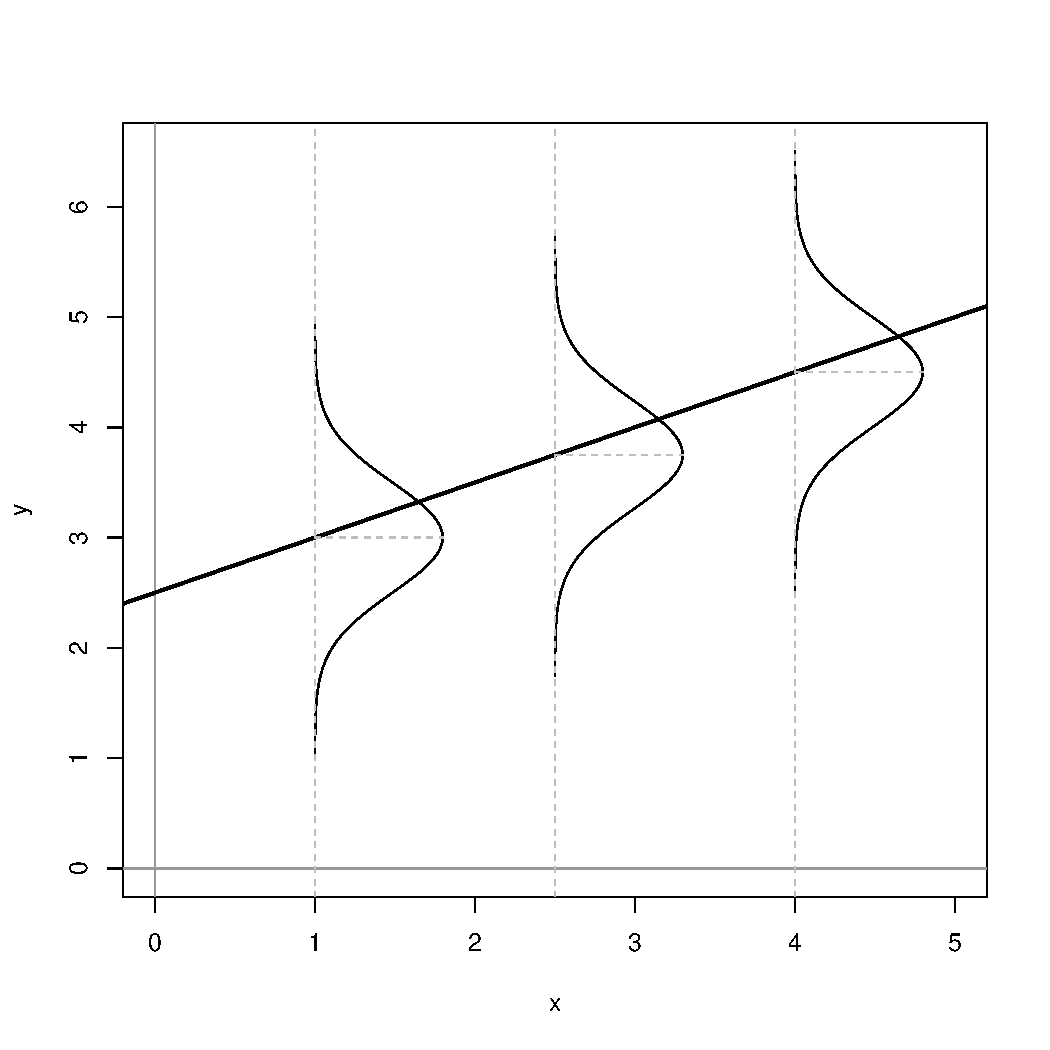
\includegraphics[width=5in, height=4in]{img/philosophy.pdf}
  \caption[Philosophical foundations of SLR]{\small Philosophical foundations of SLR.}
  \label{fig:philosophy}
\end{figure}
 


\begin{example}
\label{exa:Speed-and-Stopping}
\textbf{Speed and stopping distance of cars.} We will use the data frame \texttt{cars}\index{Data sets!cars@\texttt{cars}} from the \texttt{datasets} package. It has two variables: \texttt{speed} and \texttt{dist}. We can take a look at some of the values in the data frame: 

\begin{verbatim}
head(cars)
\end{verbatim}

\begin{verbatim}
   speed dist
 1     4    2
 2     4   10
 3     7    4
 4     7   22
 5     8   16
 6     9   10
\end{verbatim}

The \texttt{speed} represents how fast the car was going (\(x\)) in miles per hour and \texttt{dist} (\(Y\)) measures how far it took the car to stop, in feet. We can make a simple scatterplot of the data with the \texttt{qplot} command in the \texttt{ggplot2} package. 

\begin{figure}[ht!]
  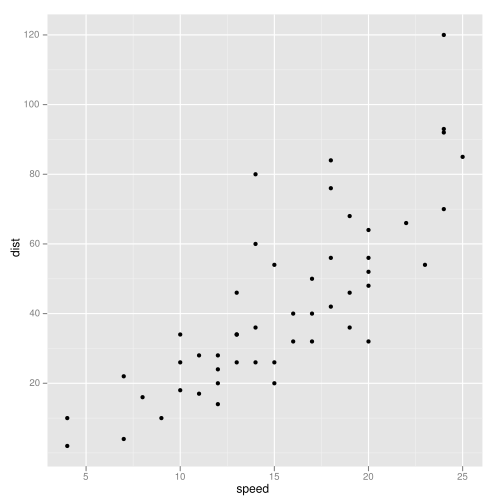
\includegraphics[width=5in, height=4in]{img/carscatter.pdf}
  \caption[Scatterplot of \texttt{dist} versus \texttt{speed} for the \texttt{cars} data]{\small A scatterplot of \texttt{dist} versus \texttt{speed} for the \texttt{cars} data.  There is clearly an upward trend to the plot which is approximately linear.}
  \label{fig:Scatter-cars}
\end{figure}


\begin{verbatim}
qplot(speed, dist, data = cars)
\end{verbatim}

You can see the output in Figure \ref{fig:Scatter-cars}, which was produced by the following code.


\begin{verbatim}
plot(dist ~ speed, data = cars)
\end{verbatim}

There is a pronounced upward trend to the data points, and the pattern looks approximately linear. There does not appear to be substantial fanning out of the points or extreme values. 
\end{example}
\section{Estimation}
\label{sec-1-2}

\label{sec:SLR-Estimation}
\subsection{Point Estimates of the Parameters}
\label{sec-1-2-1}

\label{sub:point-estimate-mle-slr}

Where is \( \mu(x) \)? In essence, we would like to ``fit'' a line to the points. But how do we determine a ``good'' line? Is there a \emph{best} line? We will use maximum likelihood\index{maximum likelihood} to find it. We know:
\begin{equation}
Y_{i} = \beta_{0} + \beta_{1}x_{i} + \epsilon_{i},\quad i=1,\ldots,n,
\end{equation}
where the \( \epsilon_{i} \) are IID \(\mathsf{norm}(\mathtt{mean}=0,\,\mathtt{sd}=\sigma) \). Thus \( Y_{i}\sim\mathsf{norm}(\mathtt{mean}=\beta_{0}+\beta_{1}x_{i},\,\mathtt{sd}=\sigma),\ i=1,\ldots,n \). Furthermore, \( Y_{1},\ldots,Y_{n} \) are independent -- but not identically distributed. The likelihood function\index{likelihood function} is:
\begin{alignat}{1}
L(\beta_{0},\beta_{1},\sigma)= & \prod_{i=1}^{n}f_{Y_{i}}(y_{i}),\\
= & \prod_{i=1}^{n}(2\pi\sigma^{2})^{-1/2}\exp\left\{ \frac{-(y_{i}-\beta_{0}-\beta_{1}x_{i})^{2}}{2\sigma^{2}}\right\} ,\\
= & (2\pi\sigma^{2})^{-n/2}\exp\left\{ \frac{-\sum_{i=1}^{n}(y_{i}-\beta_{0}-\beta_{1}x_{i})^{2}}{2\sigma^{2}}\right\} .
\end{alignat}
We take the natural logarithm to get
\begin{equation}
\ln L(\beta_{0},\beta_{1},\sigma)=-\frac{n}{2}\ln(2\pi\sigma^{2})-\frac{\sum_{i=1}^{n}(y_{i}-\beta_{0}-\beta_{1}x_{i})^{2}}{2\sigma^{2}}.\label{eq:regML-lnL}
\end{equation}
 We would like to maximize this function of \( \beta_{0} \) and \( \beta_{1} \). See Appendix \ref{sec:Multivariable-Calculus} which tells us that we should find critical points by means of the partial derivatives. Let us start by differentiating with respect to \( \beta_{0} \):
\begin{equation}
\frac{\partial}{\partial\beta_{0}}\ln L=0-\frac{1}{2\sigma^{2}}\sum_{i=1}^{n}2(y_{i}-\beta_{0}-\beta_{1}x_{i})(-1),
\end{equation}
and the partial derivative equals zero when \( \sum_{i=1}^{n}(y_{i}-\beta_{0}-\beta_{1}x_{i}) = 0 \), that is, when
\begin{equation}
n \beta_{0} + \beta_{1} \sum_{i=1}^{n} x_{i} = \sum_{i = 1}^{n}y_{i}.\label{eq:regML-a}
\end{equation}
Moving on, we next take the partial derivative of \( \ln L \) (Equation \ref{eq:regML-lnL}) with respect to \( \beta_{1} \) to get
\begin{alignat}{1}
\frac{\partial}{\partial\beta_{1}}\ln L=\  & 0-\frac{1}{2\sigma^{2}}\sum_{i=1}^{n}2(y_{i}-\beta_{0}-\beta_{1}x_{i})(-x_{i}),\\
= & \frac{1}{\sigma^{2}}\sum_{i=1}^{n}\left(x_{i}y_{i}-\beta_{0}x_{i}-\beta_{1}x_{i}^{2}\right),
\end{alignat}
and this equals zero when the last sum equals zero, that is, when
\begin{equation}
\beta_{0} \sum_{i = 1}^{n}x_{i} + \beta_{1} \sum_{i = 1}^{n}x_{i}^{2} = \sum_{i = 1}^{n}x_{i}y_{i}.\label{eq:regML-b}
\end{equation}
Solving the system of equations \ref{eq:regML-a} and \ref{eq:regML-b}
\begin{eqnarray}
n\beta_{0} + \beta_{1}\sum_{i = 1}^{n}x_{i} & = & \sum_{i = 1}^{n}y_{i}\\
\beta_{0}\sum_{i = 1}^{n}x_{i}+\beta_{1}\sum_{i = 1}^{n}x_{i}^{2} & = & \sum_{i = 1}^{n}x_{i}y_{i}
\end{eqnarray}
for \( \beta_{0} \) and \( \beta_{1} \) (in Exercise \ref{xca:find-mles-SLR}) gives
\begin{equation}
\hat{\beta}_{1} = \frac{\sum_{i = 1}^{n}x_{i}y_{i} - \left.\left(\sum_{i = 1}^{n}x_{i}\right)\left(\sum_{i = 1}^{n}y_{i}\right)\right\slash n}{\sum_{i = 1}^{n}x_{i}^{2} - \left.\left(\sum_{i = 1}^{n}x_{i}\right)^{2}\right\slash n}\label{eq:regline-slope-formula}
\end{equation}
and
\begin{equation}
\hat{\beta}_{0} = \overline{y} - \hat{\beta}_{1}\overline{x}.
\end{equation}

The conclusion? To estimate the mean line 
\begin{equation}
\mu(x) = \beta_{0} + \beta_{1}x,
\end{equation}
we use the ``line of best fit''
\begin{equation}
\hat{\mu}(x) = \hat{\beta}_{0} + \hat{\beta}_{1}x,
\end{equation}
where \(\hat{\beta}_{0}\) and \(\hat{\beta}_{1}\) are given as above. For notation we will usually write \( b_{0} = \hat{\beta_{0}} \) and \( b_{1}=\hat{\beta_{1}} \) so that \( \hat{\mu}(x) = b_{0} + b_{1}x \).

\begin{rem}
The formula for \( b_{1} \) in Equation \ref{eq:regline-slope-formula} gets the job done but does not really make any sense. There are many equivalent formulas for \( b_{1} \) that are more intuitive, or at the least are easier to remember. One of the author's favorites is
\begin{equation}
b_{1} = r\frac{s_{y}}{s_{x}},\label{eq:sample-correlation-formula}
\end{equation}
where \(r\), \( s_{y} \), and \( s_{x} \) are the sample correlation coefficient and the sample standard deviations of the \(Y\) and \(x\) data, respectively. See Exercise \ref{xca:show-alternate-slope-formula}. Also, notice the similarity between Equation \ref{eq:sample-correlation-formula} and Equation \ref{eq:population-slope-slr}.
\end{rem}

\paragraph*{How to do it with \textsf{R}}



Here we go. \textsf{R} will calculate the linear regression line with the \texttt{lm} function. We will store the result in an object which we will call \texttt{cars.lm}. Here is how it works:


\begin{verbatim}
cars.lm <- lm(dist ~ speed, data = cars)
\end{verbatim}

The first part of the input to the \texttt{lm} function, \texttt{dist \textasciitilde{} speed}, is a \emph{model formula}, read as ``\texttt{dist} is described (or modeled) by \texttt{speed}''. The \texttt{data = cars} argument tells \textsf{R} where to look for the variables quoted in the model formula. The output object \texttt{cars.lm} contains a multitude of information. Let's first take a look at the coefficients of the fitted regression line, which are extracted by the \texttt{coef} function (alternatively, we could just type \texttt{cars.lm} to see the same thing):


\begin{verbatim}
coef(cars.lm)
\end{verbatim}

\begin{verbatim}
 (Intercept)       speed 
  -17.579095    3.932409
\end{verbatim}

The parameter estimates \( b_{0} \) and \( b_{1} \) for the intercept and slope, respectively, are shown above. The regression line is thus given by \( \hat{\mu}(\mathtt{speed}) =  -17.58 +  3.93 \cdot \mathtt{speed} \).

It is good practice to visually inspect the data with the regression line added to the plot. To do this we first scatterplot the original data and hen follow with a call to the \texttt{abline} function. The inputs to \texttt{abline} are the coefficients of \texttt{cars.lm}; see Figure \ref{fig:Scatter-cars-regline}.

\begin{figure}[ht!]
  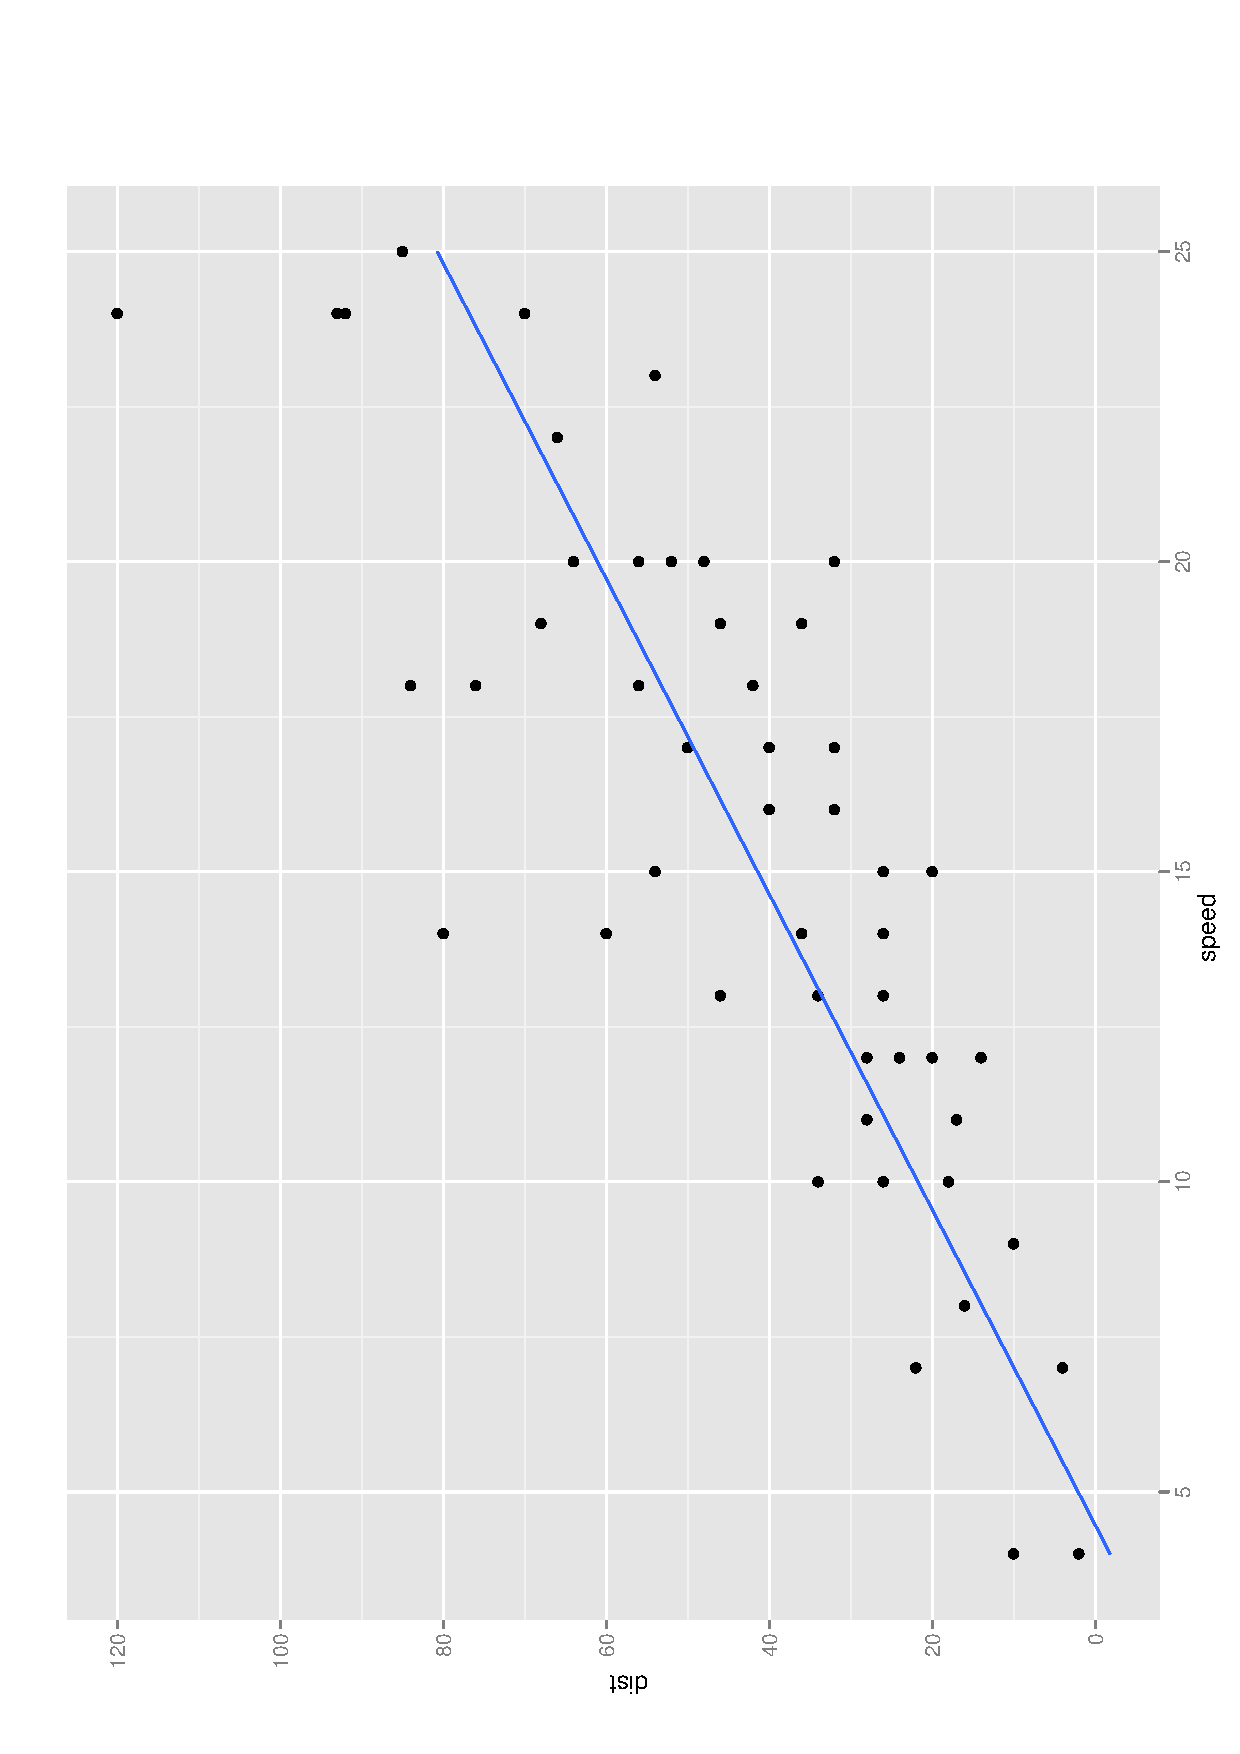
\includegraphics[width=5in, height=4in]{img/carline.pdf}
  \caption[Scatterplot with added regression line for the \texttt{cars} data]{\small A scatterplot with an added regression line for the \texttt{cars} data.}
  \label{fig:Scatter-cars-regline}
\end{figure}


\begin{verbatim}
ggplot(cars, aes(x = speed, y = dist)) + geom_point(shape = 19) + 
       geom_smooth(method = lm)
\end{verbatim}

To calculate points on the regression line we may simply plug the desired \(x\) value(s) into \( \hat{\mu} \), either by hand, or with the \texttt{predict} function. The inputs to \texttt{predict} are the fitted linear model object, \texttt{cars.lm}, and the desired \(x\) value(s) represented by a data frame. See the example below.

\begin{example}
\label{exa:regline-cars-interpret}

Using the regression line for the \texttt{cars} data:

\begin{enumerate}
\item What is the meaning of \( \mu(60) = \beta_{0} + \beta_{1}(8) \)? 
   This represents the average stopping distance (in feet) for a car going 8 mph.
\item Interpret the slope \(\beta_{1}\). 
   The true slope \(\beta_{1}\) represents the increase in average stopping distance for each mile per hour faster that the car drives. In this case, we estimate the car to take approximately \(  3.93 \) additional feet to stop for each additional mph increase in speed.
\item Interpret the intercept \( \beta_{0} \).
   This would represent the mean stopping distance for a car traveling 0 mph (which our regression line estimates to be \(  -17.58 \) ). Of course, this interpretation does not make any sense for this example, because a car travelling 0 mph takes 0 ft to stop (it was not moving in the first place)! What went wrong? Looking at the data, we notice that the smallest speed for which we have measured data is 4 mph. Therefore, if we predict what would happen for slower speeds then we would be \emph{extrapolating}, a dangerous practice which often gives nonsensical results.
\end{enumerate}
\end{example}
\subsection{Point Estimates of the Regression Line}
\label{sec-1-2-2}

\label{sub:slr-point-est-regline}

We said at the beginning of the chapter that our goal was to estimate \( \mu = \E Y \), and the arguments in Section \ref{sub:point-estimate-mle-slr} showed how to obtain an estimate \( \hat{\mu} \) of \( \mu \) when the regression assumptions hold. Now we will reap the benefits of our work in more ways than we previously disclosed. Given a particular value \(x_{0}\), there are two values we would like to estimate:
\begin{enumerate}
\item the mean value of \(Y\) at \(x_{0}\), and
\item a future value of \(Y\) at \(x_{0}\).
\end{enumerate}
The first is a number, \(\mu(x_{0})\), and the second is a random variable, \(Y(x_{0})\), but our point estimate is the same for both: \(\hat{\mu}(x_{0})\).

\begin{example}
\label{exa:regline-cars-pe-8mph}
We may use the regression line to obtain a point estimate of the mean stopping distance for a car traveling 8 mph: \( \hat{\mu}(15) = b_{0} + (8) (b_{1}) \approx  -17.58 + (8) (  3.93 ) \approx 13.88 \). We would also use 13.88 as a point estimate for the stopping distance of a future car traveling 8 mph. 
\end{example}

Note that we actually have observed data for a car traveling 8 mph; its stopping distance was 16 ft as listed in the fifth row of the \texttt{cars} data (which we saw in Example \ref{exa:Speed-and-Stopping}).


\begin{verbatim}
cars[5, ]
\end{verbatim}

\begin{verbatim}
 [1] 3.93
 [1] -17.58
 [1] -17.58
 [1] 3.93
   speed dist
 5     8   16
\end{verbatim}

There is a special name for estimates \( \hat{\mu}(x_{0}) \) when \( x_{0} \) matches an observed value \(x_{i}\) from the data set. They are called \emph{fitted values}, they are denoted by \(\hat{Y}_{1}\), \(\hat{Y}_{2}\), \ldots{}, \(\hat{Y}_{n}\) (ignoring repetition), and they play an important role in the sections that follow. 

In an abuse of notation we will sometimes write \(\hat{Y}\) or \(\hat{Y}(x_{0})\) to denote a point on the regression line even when \(x_{0}\) does not belong to the original data if the context of the statement obviates any danger of confusion.

We saw in Example \ref{exa:regline-cars-interpret} that spooky things can happen when we are cavalier about point estimation. While it is usually acceptable to predict/estimate at values of \(x_{0}\) that fall within the range of the original \(x\) data, it is reckless to use \(\hat{\mu}\) for point estimates at locations outside that range. Such estimates are usually worthless. \emph{Do not extrapolate} unless there are compelling external reasons, and even then, temper it with a good deal of caution.


\paragraph*{How to do it with \textsf{R}}

The fitted values are automatically computed as a byproduct of the model fitting procedure and are already stored as a component of the \texttt{cars.lm} object. We may access them with the \texttt{fitted} function (we only show the first five entries):


\begin{verbatim}
fitted(cars.lm)[1:5]
\end{verbatim}

\begin{verbatim}
         1         2         3         4         5 
 -1.849460 -1.849460  9.947766  9.947766 13.880175
\end{verbatim}

Predictions at \(x\) values that are not necessarily part of the original data are done with the \texttt{predict} function. The first argument is the original \texttt{cars.lm} object and the second argument \texttt{newdata} accepts a dataframe (in the same form that was used to fit \texttt{cars.lm}) that contains the locations at which we are seeking predictions. Let us predict the average stopping distances of cars traveling 6 mph, 8 mph, and 21 mph:


\begin{verbatim}
predict(cars.lm, newdata = data.frame(speed = c(6, 8, 21)))
\end{verbatim}

\begin{verbatim}
         1         2         3 
  6.015358 13.880175 65.001489
\end{verbatim}

Note that there were no observed cars that traveled 6 mph or 21 mph. Also note that our estimate for a car traveling 8 mph matches the value we computed by hand in Example \ref{exa:regline-cars-pe-8mph}.
\subsection{Mean Square Error and Standard Error}
\label{sec-1-2-3}


To find the MLE of \(\sigma^{2}\) we consider the partial derivative
\begin{equation}
\frac{\partial}{\partial\sigma^{2}}\ln L=\frac{n}{2\sigma^{2}}-\frac{1}{2(\sigma^{2})^{2}}\sum_{i=1}^{n}(y_{i}-\beta_{0}-\beta_{1}x_{i})^{2},
\end{equation}
and after plugging in \(\hat{\beta}_{0}\) and \(\hat{\beta}_{1}\) and setting equal to zero we get
\begin{equation}
\hat{\sigma^{2}}=\frac{1}{n}\sum_{i=1}^{n}(y_{i}-\hat{\beta}_{0}-\hat{\beta}_{1}x_{i})^{2}=\frac{1}{n}\sum_{i=1}^{n}[y_{i}-\hat{\mu}(x_{i})]^{2}.
\end{equation}
We write \(\hat{Yi}=\hat{\mu}(x_{i})\), and we let \(E_{i}=Y_{i}-\hat{Y_{i}}\) be the \(i^{\mathrm{th}}\) \emph{residual}. We see 
\begin{equation}
n\hat{\sigma^{2}}=\sum_{i=1}^{n}E_{i}^{2}=SSE=\mbox{ the sum of squared errors.}
\end{equation}
For a point estimate of \(\sigma^{2}\) we use the \emph{mean square error} \(S^{2}\) defined by 
\begin{equation}
S^{2}=\frac{SSE}{n-2},
\end{equation}
and we estimate \(\sigma\) with the \emph{standard error}
\footnote{Be careful not to confuse the mean square error \(S^{2}\) with the sample variance \(S^{2}\) in Chapter \ref{cha:Describing-Data-Distributions}. Other notation the reader may encounter is the lowercase \(s^{2}\) or the bulky \(MSE\).}
\(S=\sqrt{S^{2}}\).

\paragraph*{How to do it with \textsf{R}}

The residuals for the model may be obtained with the \texttt{residuals} function; we only show the first few entries in the interest of space:


\begin{verbatim}
residuals(cars.lm)[1:5]
\end{verbatim}

\begin{verbatim}
         1         2         3         4         5 
  3.849460 11.849460 -5.947766 12.052234  2.119825
\end{verbatim}



In the last section, we calculated the fitted value for \(x=8\) and found it to be approximately \( \hat{\mu}(8)\approx  13.88 \). Now, it turns out that there was only one recorded observation at \(x = 8\), and we have seen this value in the output of \texttt{head(cars)} in Example \ref{exa:Speed-and-Stopping}; it was \(\mathtt{dist} = 16\) ft for a car with \( \mathtt{speed} = 8 \) mph. Therefore, the residual should be \(E = Y - \hat{Y}\) which is \(E \approx 16 -  13.88 \). Now take a look at the last entry of \texttt{residuals(cars.lm)}, above. It is not a coincidence.

The estimate \(S\) for \(\sigma\) is called the \texttt{Residual standard error} and for the \texttt{cars} data is shown a few lines up on the \texttt{summary(cars.lm)} output (see How to do it with \textsf{R} in Section \ref{sub:slr-interval-est-params}). We may read it from there to be \( S\approx  15.38 \), or we can access it directly from the \texttt{summary} object.


\begin{verbatim}
carsumry <- summary(cars.lm)
carsumry$sigma
\end{verbatim}

\begin{verbatim}
 [1] 13.88
 [1] 13.88
 [1] 15.38
 [1] 15.37959
\end{verbatim}
\subsection{Interval Estimates of the Parameters}
\label{sec-1-2-4}

\label{sub:slr-interval-est-params}

We discussed general interval estimation in Chapter \ref{cha:Estimation}. There we found that we could use what we know about the sampling distribution of certain statistics to construct confidence intervals for the parameter being estimated. We will continue in that vein, and to get started we will determine the sampling distributions of the parameter estimates, \(b_{1}\) and \(b_{0}\).

To that end, we can see from Equation \ref{eq:regline-slope-formula} (and it is made clear in Chapter \ref{cha:multiple-linear-regression}) that \(b_{1}\) is just a linear combination of normally distributed random variables, so \(b_{1}\) is normally distributed too. Further, it can be shown that
\begin{equation}
b_{1}\sim\mathsf{norm}\left(\mathtt{mean}=\beta_{1},\,\mathtt{sd}=\sigma_{b_{1}}\right)
\end{equation}
where
\begin{equation}
\sigma_{b_{1}}=\frac{\sigma}{\sqrt{\sum_{i=1}^{n}(x_{i}-\overline{x})^{2}}}
\end{equation}
is called \emph{the standard error of} \(b_{1}\) which unfortunately depends on the unknown value of \(\sigma\). We do not lose heart, though, because we can estimate \(\sigma\) with the standard error \(S\) from the last section. This gives us an estimate \(S_{b_{1}}\) for \(\sigma_{b_{1}}\) defined by
\begin{equation}
S_{b_{1}}=\frac{S}{\sqrt{\sum_{i=1}^{n}(x_{i}-\overline{x})^{2}}}.
\end{equation}

Now, it turns out that \(b_{0}\), \(b_{1}\), and \(S\) are mutually independent (see the footnote in Section \ref{sub:mlr-interval-est-params}). Therefore, the quantity
\begin{equation}
T=\frac{b_{1}-\beta_{1}}{S_{b_{1}}}
\end{equation}
has a \(\mathsf{t}(\mathtt{df}=n-2)\) distribution and a \(100(1 - \alpha)\% \) confidence interval for \(\beta_{1}\) is given by 
\begin{equation}
b_{1}\pm\mathsf{t}_{\alpha/2}(\mathtt{df}=n-1)\, S_{b_{1}.}
\end{equation}

It is also sometimes of interest to construct a confidence interval for \(\beta_{0}\) in which case we will need the sampling distribution of \(b_{0}\). It is shown in Chapter \ref{cha:multiple-linear-regression} that
\begin{equation}
b_{0}\sim\mathsf{norm}\left(\mathtt{mean}=\beta_{0},\,\mathtt{sd}=\sigma_{b_{0}}\right),
\end{equation}
where \(\sigma_{b_{0}}\) is given by
\begin{equation}
\sigma_{b_{0}}=\sigma\sqrt{\frac{1}{n}+\frac{\overline{x}^{2}}{\sum_{i=1}^{n}(x_{i}-\overline{x})^{2}}},
\end{equation}
and which we estimate with the \(S_{b_{0}}\) defined by
\begin{equation}
S_{b_{0}}=S\sqrt{\frac{1}{n}+\frac{\overline{x}^{2}}{\sum_{i=1}^{n}(x_{i}-\overline{x})^{2}}}.
\end{equation}
Thus the quantity
\begin{equation}
T=\frac{b_{0}-\beta_{0}}{S_{b_{0}}}
\end{equation}
has a \(\mathsf{t}(\mathtt{df}=n-2)\) distribution and a \(100(1-\alpha)\%\) confidence interval for \(\beta_{0}\) is given by
\begin{equation}
b_{0}\pm\mathsf{t}_{\alpha/2}(\mathtt{df}=n-1)\, S_{b_{0}}.
\end{equation}

\paragraph*{How to do it with \textsf{R}}



Let us take a look at the output from \texttt{summary(cars.lm)}:


\begin{verbatim}
summary(cars.lm)
\end{verbatim}


\begin{verbatim}
 
Call:
lm(formula = dist ~ speed, data = cars)

Residuals:
    Min      1Q  Median      3Q     Max 
-29.069  -9.525  -2.272   9.215  43.201 

Coefficients:
            Estimate Std. Error t value Pr(>|t|)    
(Intercept) -17.5791     6.7584  -2.601   0.0123 *  
speed         3.9324     0.4155   9.464 1.49e-12 ***
---
Signif. codes:  0 '***' 0.001 '**' 0.01 '*' 0.05 '.' 0.1 ' ' 1 

Residual standard error: 15.38 on 48 degrees of freedom
Multiple R-squared: 0.6511,	Adjusted R-squared: 0.6438 
F-statistic: 89.57 on 1 and 48 DF,  p-value: 1.49e-12
\end{verbatim}

In the \texttt{Coefficients} section we find the parameter estimates and their respective standard errors in the second and third columns; the other columns are discussed in Section \ref{sec:Model-Utility-SLR}. If we wanted, say, a 95\% confidence interval for \(\beta_{1}\) we could use \( b_{1} =  3.932 \) and \( S_{b_{1}} =  0.416 \) together with a \( \mathsf{t}_{0.025}(\mathtt{df}=23) \) critical value to calculate \( b_{1} \pm \mathsf{t}_{0.025}(\mathtt{df} = 23) \cdot S_{b_{1}} \).  Or, we could use the \texttt{confint} function.


\begin{verbatim}
confint(cars.lm)
\end{verbatim}

\begin{verbatim}
 [1] 3.932
 [1] 0.416
                  2.5 %    97.5 %
 (Intercept) -31.167850 -3.990340
 speed         3.096964  4.767853
\end{verbatim}

With 95\% confidence, the random interval \( [  3.097,  4.768 ] \) covers the parameter \(\beta_{1}\).
\subsection{Interval Estimates of the Regression Line}
\label{sec-1-2-5}

\label{sub:slr-interval-est-regline}

We have seen how to estimate the coefficients of regression line with both point estimates and confidence intervals. We even saw how to estimate a value \(\hat{\mu}(x)\) on the regression line for a given value of \(x\), such as \(x=15\). 

But how good is our estimate \(\hat{\mu}(15)\)? How much confidence do we have in \emph{this} estimate? Furthermore, suppose we were going to observe another value of \(Y\) at \(x=15\). What could we say?

Intuitively, it should be easier to get bounds on the mean (average) value of \(Y\) at \(x_{0}\) -- called a \emph{confidence interval for the mean value of} \(Y\) \emph{at} \(x_{0}\) -- than it is to get bounds on a future observation of \(Y\) (called a \emph{prediction interval for \(Y\) at \(x_{0}\)}). As we shall see, the intuition serves us well and confidence intervals are shorter for the mean value, longer for the individual value.

Our point estimate of \(\mu(x_{0})\) is of course \(\hat{Y}=\hat{Y}(x_{0})\), so for a confidence interval we will need to know \(\hat{Y}\)'s sampling distribution. It turns out (see Section ) that \(\hat{Y}=\hat{\mu}(x_{0})\) is distributed
\begin{equation}
\hat{Y}\sim\mathsf{norm}\left(\mathtt{mean}=\mu(x_{0}),\:\mathtt{sd}=\sigma\sqrt{\frac{1}{n}+\frac{(x_{0}-\overline{x})^{2}}{\sum_{i=1}^{n}(x_{i}-\overline{x})^{2}}}\right).
\end{equation}

Since \(\sigma\) is unknown we estimate it with \(S\) (we should expect the appearance of a \(\mathsf{t}(\mathtt{df}=n-2)\) distribution in the near future). 

A \( 100(1-\alpha)\% \) \emph{confidence interval (CI) for} \(\mu(x_{0})\) is given by
\begin{equation}
\hat{Y}\pm\mathsf{t}_{\alpha/2}(\mathtt{df}=n-2)\, S\sqrt{\frac{1}{n}+\frac{(x_{0}-\overline{x}^{2})}{\sum_{i=1}^{n}(x_{i}-\overline{x})^{2}}}.\label{eq:SLR-conf-int-formula}
\end{equation}
Prediction intervals are a little bit different. In order to find confidence bounds for a new observation of \(Y\) (we will denote it \(Y_{\mbox{new}}\)) we use the fact that
\begin{equation}
Y_{\mbox{new}}\sim\mathtt{norm}\left(\mathtt{mean}=\mu(x_{0}),\,\mathtt{sd}=\sigma\sqrt{1+\frac{1}{n}+\frac{(x_{0}-\overline{x})^{2}}{\sum_{i=1}^{n}(x_{i}-\overline{x})^{2}}}\right).
\end{equation}
Of course, \(\sigma\) is unknown so we estimate it with \(S\) and a \( 100(1-\alpha)\% \) prediction interval (PI) for a future value of \(Y\) at \(x_{0}\) is given by 
\begin{equation}
\hat{Y}(x_{0})\pm\mathsf{t}_{\alpha/2}(\mathtt{df}=n-1)\: S\,\sqrt{1+\frac{1}{n}+\frac{(x_{0}-\overline{x})^{2}}{\sum_{i=1}^{n}(x_{i}-\overline{x})^{2}}}.\label{eq:SLR-pred-int-formula}
\end{equation}
We notice that the prediction interval in Equation \ref{eq:SLR-pred-int-formula} is wider than the confidence interval in Equation \ref{eq:SLR-conf-int-formula}, as we expected at the beginning of the section.


\paragraph*{How to do it with \textsf{R}}

Confidence and prediction intervals are calculated in \textsf{R} with the \texttt{predict}\index{predict@\texttt{predict}} function, which we encountered in Section \ref{sub:slr-point-est-regline}. There we neglected to take advantage of its additional \texttt{interval} argument. The general syntax follows. 

\begin{example}
We will find confidence and prediction intervals for the stopping distance of a car travelling 5, 6, and 21 mph (note from the graph that there are no collected data for these speeds). We have computed \texttt{cars.lm} earlier, and we will use this for input to the \texttt{predict} function. Also, we need to tell \textsf{R} the values of \(x_{0}\) at which we want the predictions made, and store the \(x_{0}\) values in a data frame whose variable is labeled with the correct name. \emph{This is important}. 


\begin{verbatim}
new <- data.frame(speed = c(5, 6, 21))
\end{verbatim}

\begin{verbatim}
 [1] 3.097
 [1] 4.768
\end{verbatim}

Next we instruct \textsf{R} to calculate the intervals. Confidence intervals are given by 


\begin{verbatim}
predict(cars.lm, newdata = new, interval = "confidence")
\end{verbatim}

\begin{verbatim}
         fit       lwr      upr
 1  2.082949 -7.644150 11.81005
 2  6.015358 -2.973341 15.00406
 3 65.001489 58.597384 71.40559
\end{verbatim}



Prediction intervals are given by


\begin{verbatim}
predict(cars.lm, newdata = new, interval = "prediction")
\end{verbatim}

\begin{verbatim}
         fit       lwr      upr
 1  2.082949 -30.33359 34.49948
 2  6.015358 -26.18731 38.21803
 3 65.001489  33.42257 96.58040
\end{verbatim}



\end{example}

The type of interval is dictated by the \texttt{interval} argument (which is \texttt{none} by default), and the default confidence level is 95\% (which can be changed with the \texttt{level} argument). 

\begin{example}
Using the \texttt{cars} data,
\begin{enumerate}
\item Report a point estimate of and a 95\% confidence interval for the mean stopping distance for a car travelling 5 mph.
   The fitted value for \(x=5\) is \(  2.08 \), so a point estimate would be \(  2.08 \) ft. The 95\% CI is given by \( [  -7.64,  11.81 ] \), so with 95\% confidence the mean stopping distance lies somewhere between \(  -7.64 \) ft and \(  11.81 \) ft.
\item Report a point prediction for and a 95\% prediction interval for the stopping distance of a hypothetical car travelling 21 mph.
   The fitted value for \(x = 21\) is \(  65 \), so a point prediction for the stopping distance is \(  65 \) ft. The 95\% PI is \( [  33.42,  96.58 ] \), so with 95\% confidence we may assert that the hypothetical stopping distance for a car travelling 21 mph would lie somewhere between \(  33.42 \) ft and \(  96.58 \) ft.
\end{enumerate}
\end{example}
\subsection{Graphing the Confidence and Prediction Bands}
\label{sec-1-2-6}


We earlier guessed that a bound on the value of a single new observation would be inherently less certain than a bound for an average (mean) value; therefore, we expect the CIs for the mean to be tighter than the PIs for a new observation. A close look at the standard deviations in Equations \ref{eq:SLR-conf-int-formula} and \ref{eq:SLR-pred-int-formula} confirms our guess, but we would like to see a picture to drive the point home.

We may plot the confidence and prediction intervals with one fell swoop using the \texttt{ci.plot} function from the \texttt{HH} package \cite{Heibergerhh}. The graph is displayed in Figure \ref{fig:Scatter-cars-CIPI}.

\begin{figure}[ht!]
  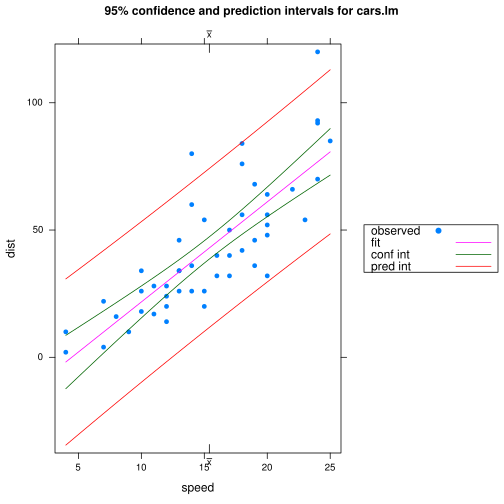
\includegraphics[width=5in, height=4in]{img/carscipi.pdf}
  \caption[Scatterplot with confidence/prediction bands for the \texttt{cars} data]{\small A scatterplot with confidence/prediction bands for the \texttt{cars} data.}
  \label{fig:Scatter-cars-CIPI}
\end{figure}


\begin{verbatim}
library(HH)
ci.plot(cars.lm)
\end{verbatim}

Notice that the bands curve outward from the regression line as the \(x\) values move away from the center. This is expected once we notice the \((x_{0}-\overline{x})^{2}\) term in the standard deviation formulas in Equations \ref{eq:SLR-conf-int-formula} and \ref{eq:SLR-pred-int-formula}.
\section{Model Utility and Inference}
\label{sec-1-3}

\label{sec:Model-Utility-SLR}
\subsection{Hypothesis Tests for the Parameters}
\label{sec-1-3-1}

\label{sub:slr-hypoth-test-params}

Much of the attention of SLR is directed toward \(\beta_{1}\) because when \( \beta_{1}\neq 0 \) the mean value of \(Y\) increases (or decreases) as \(x\) increases. It is really boring when \(\beta_{1}=0\), because in that case the mean value of \(Y\) remains the same, regardless of the value of \(x\) (when the regression assumptions hold, of course). It is thus very important to decide whether or not \( \beta_{1} = 0 \). We address the question with a statistical test of the null hypothesis \(H_{0}:\beta_{1}=0\) versus the alternative hypothesis \(H_{1}:\beta_{1}\neq0\), and to do that we need to know the sampling distribution of \(b_{1}\) when the null hypothesis is true.

To this end we already know from Section \ref{sub:slr-interval-est-params} that the quantity

\begin{equation} 
T=\frac{b_{1}-\beta_{1}}{S_{b_{1}}}
\end{equation}
has a \(\mathsf{t}(\mathtt{df}=n-2)\) distribution; therefore, when \(\beta_{1}=0\) the quantity \(b_{1}/S_{b_{1}}\) has a \(\mathsf{t}(\mathtt{df}=n-2)\) distribution and we can compute a \(p\)-value by comparing the observed value of \(b_{1}/S{}_{b_{1}}\) with values under a \(\mathsf{t}(\mathtt{df}=n-2)\) curve. 

Similarly, we may test the hypothesis \(H_{0}:\beta_{0}=0\) versus the alternative \(H_{1}:\beta_{0}\neq0\) with the statistic \(T=b_{0}/S_{b_{0}}\), where \(S_{b_{0}}\) is given in Section \ref{sub:slr-interval-est-params}. The test is conducted the same way as for \(\beta_{1}\). 


\paragraph*{How to do it with \textsf{R}}

Let us take another look at the output from \texttt{summary(cars.lm)}:


\begin{verbatim}
summary(cars.lm)
\end{verbatim}


\begin{verbatim}
null device 
          1
 
Call:
lm(formula = dist ~ speed, data = cars)

Residuals:
    Min      1Q  Median      3Q     Max 
-29.069  -9.525  -2.272   9.215  43.201 

Coefficients:
            Estimate Std. Error t value Pr(>|t|)    
(Intercept) -17.5791     6.7584  -2.601   0.0123 *  
speed         3.9324     0.4155   9.464 1.49e-12 ***
---
Signif. codes:  0 '***' 0.001 '**' 0.01 '*' 0.05 '.' 0.1 ' ' 1 

Residual standard error: 15.38 on 48 degrees of freedom
Multiple R-squared: 0.6511,	Adjusted R-squared: 0.6438 
F-statistic: 89.57 on 1 and 48 DF,  p-value: 1.49e-12
\end{verbatim}

In the \texttt{Coefficients} section we find the \(t\) statistics and the \(p\)-values associated with the tests that the respective parameters are zero in the fourth and fifth columns. Since the \(p\)-values are (much) less than 0.05, we conclude that there is strong evidence that the parameters \(\beta_{1}\neq0\) and \(\beta_{0}\neq0\), and as such, we say that there is a statistically significant linear relationship between \texttt{dist} and \texttt{speed}. 
\subsection{Simple Coefficient of Determination}
\label{sec-1-3-2}


It would be nice to have a single number that indicates how well our linear regression model is doing, and the \emph{simple coefficient of determination} is designed for that purpose. In what follows, we observe the values \(Y_{1}\), \(Y_{2}\), \ldots{},\(Y_{n}\), and the goal is to estimate \(\mu(x_{0})\), the mean value of \(Y\) at the location \(x_{0}\). 

If we disregard the dependence of \(Y\) and \(x\) and base our estimate only on the \(Y\) values then a reasonable choice for an estimator is just the MLE of \(\mu\), which is \(\overline{Y}\). Then the errors incurred by the estimate are just \(Y_{i}-\overline{Y}\) and the variation about the estimate as measured by the sample variance is proportional to
\begin{equation}
SSTO=\sum_{i=1}^{n}(Y_{i}-\overline{Y})^{2}.
\end{equation}
The acronym \(SSTO\) stands for \emph{total sum of squares}.  And we have additional information, namely, we have values \(x_{i}\) associated with each value of \(Y_{i}\). We have seen that this information leads us to the estimate \(\hat{Y_{i}}\) and the errors incurred are just the residuals, \(E_{i}=Y_{i}-\hat{Y_{i}}\). The variation associated with these errors can be measured with 
\begin{equation}
SSE=\sum_{i=1}^{n}(Y_{i}-\hat{Y_{i}})^{2}.
\end{equation}
We have seen the \(SSE\) before, which stands for the \emph{sum of squared errors} or \emph{error sum of squares}. Of course, we would expect the error to be less in the latter case, since we have used more information. The improvement in our estimation as a result of the linear regression model can be measured with the difference
\[
(Y_{i}-\overline{Y})-(Y_{i}-\hat{Y_{i}})=\hat{Y_{i}}-\overline{Y},
\]
and we measure the variation in these errors with
\begin{equation}
SSR=\sum_{i=1}^{n}(\hat{Y_{i}}-\overline{Y})^{2},
\end{equation}
also known as the \emph{regression sum of squares}. It is not obvious, but some algebra proved a famous result known as the \textbf{ANOVA Equality}:
\begin{equation}
\sum_{i=1}^{n}(Y_{i}-\overline{Y})^{2}=\sum_{i=1}^{n}(\hat{Y_{i}}-\overline{Y})^{2}+\sum_{i=1}^{n}(Y_{i}-\hat{Y_{i}})^{2}\label{eq:anovaeq}
\end{equation}
or in other words,
\begin{equation}
SSTO=SSR+SSE.
\end{equation}
This equality has a nice interpretation. Consider \(SSTO\) to be the \emph{total variation} of the errors. Think of a decomposition of the total variation into pieces: one piece measuring the reduction of error from using the linear regression model, or \emph{explained variation} (\(SSR\)), while the other represents what is left over, that is, the errors that the linear regression model doesn't explain, or \emph{unexplained variation} (\(SSE\)). In this way we see that the ANOVA equality merely partitions the variation into 
\[
\mbox{total variation}=\mbox{explained variation}+\mbox{unexplained variation}.
\]
For a single number to summarize how well our model is doing we use the \emph{simple coefficient of determination} \(r^{2}\), defined by
\begin{equation}
r^{2}=1-\frac{SSE}{SSTO}.
\end{equation}
We interpret \(r^{2}\) as the proportion of total variation that is explained by the simple linear regression model. When \(r^{2}\) is large, the model is doing a good job; when \(r^{2}\) is small, the model is not doing a good job.

Related to the simple coefficient of determination is the sample correlation coefficient, \(r\). As you can guess, the way we get \(r\) is by the formula \(|r|=\sqrt{r^{2}}\). The sign of \(r\) is equal the sign of the slope estimate \(b_{1}\). That is, if the regression line \(\hat{\mu}(x)\) has positive slope, then \(r=\sqrt{r^{2}}\). Likewise, if the slope of \(\hat{\mu}(x)\) is negative, then \(r=-\sqrt{r^{2}}\).


\paragraph*{How to do it with \textsf{R}}

The primary method to display partitioned sums of squared errors is with an \emph{ANOVA table}. The command in \textsf{R} to produce such a table is \texttt{anova}. The input to \texttt{anova} is the result of an \texttt{lm} call which for the \texttt{cars} data is \texttt{cars.lm}.


\begin{verbatim}
anova(cars.lm)
\end{verbatim}

\begin{verbatim}
 Analysis of Variance Table
 
 Response: dist
           Df Sum Sq Mean Sq F value   Pr(>F)    
 speed      1  21186 21185.5  89.567 1.49e-12 ***
 Residuals 48  11354   236.5                     
 ---
 Signif. codes:  0 '***' 0.001 '**' 0.01 '*' 0.05 '.' 0.1 ' ' 1
\end{verbatim}

The output gives
\[
r^{2}=1-\frac{SSE}{SSR+SSE}=1-\frac{11353.5}{21185.5+11353.5}\approx0.65.
\]

The interpretation should be: ``The linear regression line accounts for approximately 65\% of the variation of \texttt{dist} as explained by \texttt{speed}''.

The value of \(r^{2}\) is stored in the \texttt{r.squared} component of \texttt{summary(cars.lm)}, which we called \texttt{carsumry}.


\begin{verbatim}
carsumry$r.squared
\end{verbatim}

\begin{verbatim}
 [1] 0.6510794
\end{verbatim}

We already knew this. We saw it in the next to the last line of the \texttt{summary(cars.lm)} output where it was called \texttt{Multiple R-squared}. Listed right beside it is the \texttt{Adjusted R-squared} which we will discuss in Chapter \ref{cha:multiple-linear-regression}.  For the \texttt{cars} data, we find \(r\) to be


\begin{verbatim}
sqrt(carsumry$r.squared)
\end{verbatim}

\begin{verbatim}
 [1] 0.8068949
\end{verbatim}

We choose the principal square root because the slope of the regression line is positive.
\subsection{Overall \emph{F} statistic}
\label{sec-1-3-3}

\label{sub:slr-overall-F-statistic}

There is another way to test the significance of the linear regression model. In SLR, the new way also tests the hypothesis \(H_{0}:\beta_{1}=0\) versus \(H_{1}:\beta_{1}\neq0\), but it is done with a new test statistic called the \emph{overall F statistic}. It is defined by

\begin{equation}
F=\frac{SSR}{SSE/(n-2)}.\label{eq:slr-overall-F-statistic}
\end{equation}

Under the regression assumptions and when \(H_{0}\) is true, the \(F\) statistic has an \(\mathtt{f}(\mathtt{df1}=1,\,\mathtt{df2}=n-2)\) distribution. We reject \(H_{0}\) when \(F\) is large -- that is, when the explained variation is large relative to the unexplained variation.

All this being said, we have not yet gained much from the overall \(F\) statistic because we already knew from Section \ref{sub:slr-hypoth-test-params} how to test \(H_{0}:\beta_{1}=0\)\ldots{} we use the Student's \(t\) statistic. What is worse is that (in the simple linear regression model) it can be proved that the \(F\) in Equation \ref{eq:slr-overall-F-statistic} is exactly the Student's \(t\) statistic for \(\beta_{1}\) squared,

\begin{equation}
F=\left(\frac{b_{1}}{S_{b_{1}}}\right)^{2}.
\end{equation}

So why bother to define the \(F\) statistic? Why not just square the \(t\) statistic and be done with it? The answer is that the \(F\) statistic has a more complicated interpretation and plays a more important role in the multiple linear regression model which we will study in Chapter \ref{cha:multiple-linear-regression}. See Section \ref{sub:mlr-Overall-F-Test} for details.

\paragraph*{How to do it with \textsf{R}}

The overall \(F\) statistic and \(p\)-value are displayed in the bottom line of the \texttt{summary(cars.lm)} output. It is also shown in the final columns of \texttt{anova(cars.lm)}:


\begin{verbatim}
anova(cars.lm)
\end{verbatim}

\begin{verbatim}
 Analysis of Variance Table
 
 Response: dist
           Df Sum Sq Mean Sq F value   Pr(>F)    
 speed      1  21186 21185.5  89.567 1.49e-12 ***
 Residuals 48  11354   236.5                     
 ---
 Signif. codes:  0 '***' 0.001 '**' 0.01 '*' 0.05 '.' 0.1 ' ' 1
\end{verbatim}



Here we see that the \(F\) statistic is \(  89.57 \) with a \(p\)-value very close to zero. The conclusion: there is very strong evidence that \(H_{0}:\beta_{1} = 0 \) is false, that is, there is strong evidence that \( \beta_{1} \neq 0 \). Moreover, we conclude that the regression relationship between \texttt{dist} and \texttt{speed} is significant.

Note that the value of the \(F\) statistic is the same as the Student's \(t\) statistic for \texttt{speed} squared.
\section{Residual Analysis}
\label{sec-1-4}

\label{sec:Residual-Analysis-SLR}

We know from our model that \(Y=\mu(x)+\epsilon\), or in other words, \(\epsilon=Y-\mu(x)\). Further, we know that \(\epsilon\sim\mathsf{norm}(\mathtt{mean}=0,\,\mathtt{sd}=\sigma)\). We may estimate \(\epsilon_{i}\) with the \emph{residual} \(E_{i}=Y_{i}-\hat{Y_{i}}\), where \(\hat{Y_{i}}=\hat{\mu}(x_{i})\). If the regression assumptions hold, then the residuals should be normally distributed. We check this in Section \ref{sub:Normality-Assumption}. Further, the residuals should have mean zero with constant variance \(\sigma^{2}\), and we check this in Section \ref{sub:Constant-Variance-Assumption}. Last, the residuals should be independent, and we check this in Section \ref{sub:Independence-Assumption}.

In every case, we will begin by looking at residual plots -- that is, scatterplots of the residuals \(E_{i}\) versus index or predicted values \(\hat{Y_{i}}\) -- and follow up with hypothesis tests.
\subsection{Normality Assumption}
\label{sec-1-4-1}

\label{sub:Normality-Assumption}

We can assess the normality of the residuals with graphical methods and hypothesis tests. To check graphically whether the residuals are normally distributed we may look at histograms or \emph{q-q} plots. We first examine a histogram in Figure \ref{fig:Normal-q-q-plot-cars}. There we see that the distribution of the residuals appears to be mound shaped, for the most part. We can plot the order statistics of the sample versus quantiles from a \(\mathsf{norm}(\mathtt{mean}=0,\,\mathtt{sd}=1)\) distribution with the command \texttt{plot(cars.lm, which = 2)}, and the results are in Figure \ref{fig:Normal-q-q-plot-cars}. If the assumption of normality were true, then we would expect points randomly scattered about the dotted straight line displayed in the figure. In this case, we see a slight departure from normality in that the dots show systematic clustering on one side or the other of the line. The points on the upper end of the plot also appear begin to stray from the line. We would say there is some evidence that the residuals are not perfectly normal. 

\begin{figure}[ht!]
  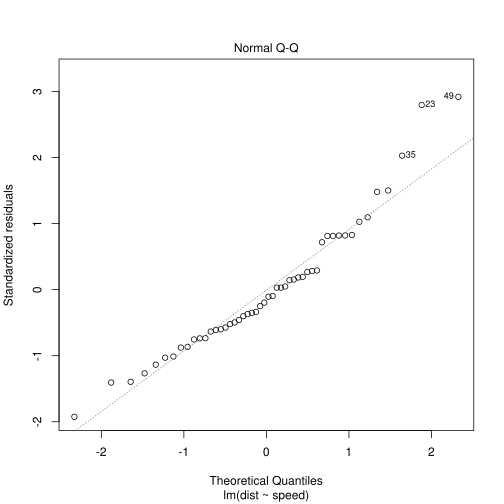
\includegraphics[width=5in, height=4in]{img/Normal-q-q-plot-cars.pdf}
  \caption[Normal q-q plot of the residuals for the \texttt{cars} data]{\small Used for checking the normality assumption. Look out for
any curvature or substantial departures from the straight line; hopefully
the dots hug the line closely.}
  \label{fig:Normal-q-q-plot-cars}
\end{figure}


\begin{verbatim}
plot(cars.lm, which = 2)
\end{verbatim}


\paragraph*{Testing the Normality Assumption}

Even though we may be concerned about the plots, we can use tests to determine if the evidence present is statistically significant, or if it could have happened merely by chance. There are many statistical tests of normality. We will use the Shapiro-Wilk test, since it is known to be a good test and to be quite powerful. However, there are many other fine tests of normality including the Anderson-Darling test and the Lillefors test, just to mention two of them.  


The Shapiro-Wilk test is based on the statistic
\begin{equation}
W=\frac{\left(\sum_{i=1}^{n}a_{i}E_{(i)}\right)^{2}}{\sum_{j=1}^{n}E_{j}^{2}},
\end{equation}
where the \(E_{(i)}\) are the ordered residuals and the \(a_{i}\) are constants derived from the order statistics of a sample of size \(n\) from a normal distribution. See Section \ref{sub:Shapiro-Wilk-Normality-Test}.
We perform the Shapiro-Wilk test below, using the \texttt{shapiro.test} function from the \texttt{stats} package. The hypotheses are
\[
H_{0}:\mbox{ the residuals are normally distributed }
\]
versus
\[
H_{1}:\mbox{ the residuals are not normally distributed.}
\]
The results from \textsf{R} are


\begin{verbatim}
shapiro.test(residuals(cars.lm))
\end{verbatim}

\begin{verbatim}
 null device 
           1
  
 	Shapiro-Wilk normality test
 
 data:  residuals(cars.lm) 
 W = 0.9451, p-value = 0.02153
\end{verbatim}

For these data we would reject the assumption of normality of the residuals at the \(\alpha=0.05\) significance level, but do not lose heart, because the regression model is reasonably robust to departures from the normality assumption. As long as the residual distribution is not highly skewed, then the regression estimators will perform reasonably well. Moreover, departures from constant variance and independence will sometimes affect the quantile plots and histograms, therefore it is wise to delay final decisions regarding normality until all diagnostic measures have been investigated.
\subsection{Constant Variance Assumption}
\label{sec-1-4-2}

\label{sub:Constant-Variance-Assumption}

We will again go to residual plots to try and determine if the spread of the residuals is changing over time (or index). However, it is unfortunately not that easy because the residuals do not have constant variance! In fact, it can be shown that the variance of the residual \(E_{i}\) is 
\begin{equation}
\mbox{Var\ensuremath{(E_{i})}}=\sigma^{2}(1-h_{ii}),\quad i=1,2,\ldots,n,
\end{equation}
where \(h_{ii}\) is a quantity called the \emph{leverage} which is defined below. Consequently, in order to check the constant variance assumption we must standardize the residuals before plotting. We estimate the standard error of \(E_{i}\) with \(s_{E_{i}}=s\sqrt{(1-h_{ii})}\) and define the \emph{standardized residuals} \(R_{i}\), \(i=1,2,\ldots,n\), by 
\begin{equation} 
R_{i}=\frac{E_{i}}{s\,\sqrt{1-h_{ii}}},\quad i=1,2,\ldots,n.
\end{equation}
For the constant variance assumption we do not need the sign of the residual so we will plot \(\sqrt{|R_{i}|}\) versus the fitted values. As we look at a scatterplot of \(\sqrt{|R_{i}|}\) versus \(\hat{Y}_{i}\) we would expect under the regression assumptions to see a constant band of observations, indicating no change in the magnitude of the observed distance from the line. We want to watch out for a fanning-out of the residuals, or a less common funneling-in of the residuals. Both patterns indicate a change in the residual variance and a consequent departure from the regression assumptions, the first an increase, the second a decrease.

In this case, we plot the standardized residuals versus the fitted values. The graph may be seen in Figure \ref{fig:std-resids-fitted-cars}. For these data there does appear to be somewhat of a slight fanning-out of the residuals.

\begin{figure}[ht!]
  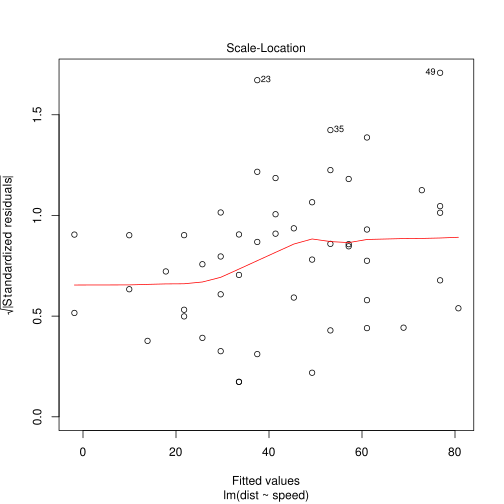
\includegraphics[width=5in, height=4in]{img/std-resids-fitted-cars.pdf}
  \caption[Plot of standardized residuals against the fitted values for the \texttt{cars} data]{\small Used for checking the constant variance assumption. Watch out for any fanning out (or in) of the dots; hopefully they fall in a constant band.}
  \label{fig:std-resids-fitted-cars}
\end{figure}


\begin{verbatim}
plot(cars.lm, which = 3)
\end{verbatim}

\paragraph*{Testing the Constant Variance Assumption}

We will use the Breusch-Pagan test to decide whether the variance of the residuals is nonconstant. The null hypothesis is that the variance is the same for all observations, and the alternative hypothesis is that the variance is not the same for all observations. The test statistic is found by fitting a linear model to the centered squared residuals,
\begin{equation}
W_{i} = E_{i}^{2} - \frac{SSE}{n}, \quad i=1,2,\ldots,n.
\end{equation}

By default the same explanatory variables are used in the new model which produces fitted values \(\hat{W}_{i}\), \(i=1,2,\ldots,n\). The Breusch-Pagan test statistic in \textsf{R} is then calculated with 
\begin{equation}
BP=n\sum_{i=1}^{n}\hat{W}_{i}^{2}\div\sum_{i=1}^{n}W_{i}^{2}.
\end{equation}
We reject the null hypothesis if \(BP\) is too large, which happens when the explained variation i the new model is large relative to the unexplained variation in the original model.
We do it in \textsf{R} with the \texttt{bptest} function from the \texttt{lmtest} package \cite{Zeileislmtest}. 

\begin{verbatim}
library(lmtest)
bptest(cars.lm)
\end{verbatim}

\begin{verbatim}
 null device 
           1
  
 	studentized Breusch-Pagan test
 
 data:  cars.lm 
 BP = 3.2149, df = 1, p-value = 0.07297
\end{verbatim}

For these data we would not reject the null hypothesis at the \(\alpha=0.05\) level. There is relatively weak evidence against the assumption of constant variance. 
\subsection{Independence Assumption}
\label{sec-1-4-3}

\label{sub:Independence-Assumption}

One of the strongest of the regression assumptions is the one regarding independence. Departures from the independence assumption are often exhibited by correlation (or autocorrelation, literally, self-correlation) present in the residuals. There can be positive or negative correlation.

Positive correlation is displayed by positive residuals followed by positive residuals, and negative residuals followed by negative residuals. Looking from left to right, this is exhibited by a cyclical feature in the residual plots, with long sequences of positive residuals being followed by long sequences of negative ones.

On the other hand, negative correlation implies positive residuals followed by negative residuals, which are then followed by positive residuals, \emph{etc}. Consequently, negatively correlated residuals are often associated with an alternating pattern in the residual plots. We examine the residual plot in Figure \ref{fig:resids-fitted-cars}. There is no obvious cyclical wave pattern or structure to the residual plot. 

\begin{figure}[ht!]
  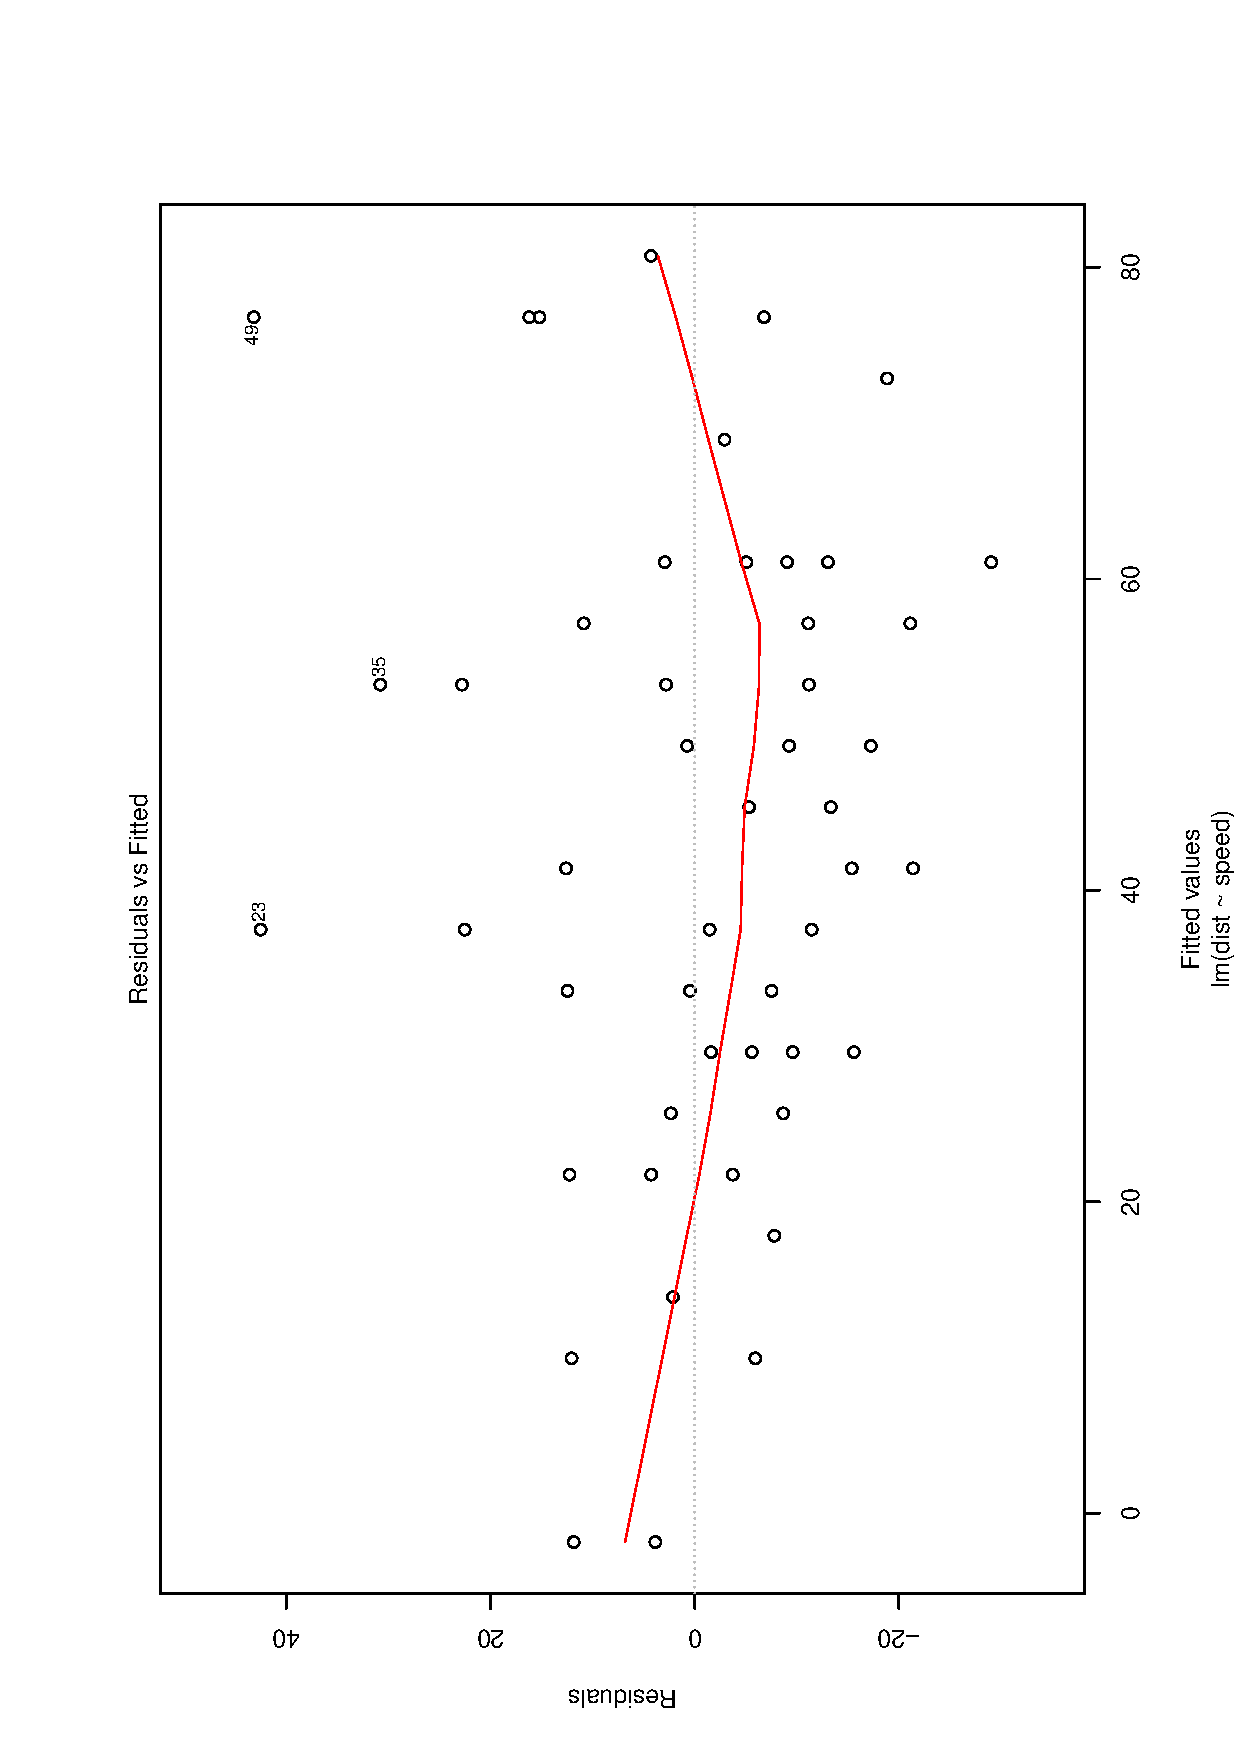
\includegraphics[width=5in, height=4in]{img/resids-fitted-cars.pdf}
  \caption[Plot of the residuals versus the fitted values for the \texttt{cars}
data]{\small Used for checking the independence assumption. Watch out for any patterns or structure; hopefully the points are randomly scattered on the plot.}
  \label{fig:resids-fitted-cars}
\end{figure}


\begin{verbatim}
plot(cars.lm, which = 1)
\end{verbatim}

\paragraph*{Testing the Independence Assumption}

We may statistically test whether there is evidence of autocorrelation in the residuals with the Durbin-Watson test. The test is based on the statistic
\begin{equation}
D=\frac{\sum_{i=2}^{n}(E_{i}-E_{i-1})^{2}}{\sum_{j=1}^{n}E_{j}^{2}}.
\end{equation}
Exact critical values are difficult to obtain, but \textsf{R} will calculate the \emph{p-value} to great accuracy. It is performed with the \texttt{dwtest} function from the \texttt{lmtest} package. We will conduct a two sided test that the correlation is not zero, which is not the default (the default is to test that the autocorrelation is positive).


\begin{verbatim}
library(lmtest)
dwtest(cars.lm, alternative = "two.sided")
\end{verbatim}

\begin{verbatim}
 null device 
           1
  
 	Durbin-Watson test
 
 data:  cars.lm 
 DW = 1.6762, p-value = 0.1904
 alternative hypothesis: true autocorrelation is not 0
\end{verbatim}

In this case we do not reject the null hypothesis at the \(\alpha=0.05\) significance level; there is very little evidence of nonzero autocorrelation in the residuals.
\subsection{Remedial Measures}
\label{sec-1-4-4}


We often find problems with our model that suggest that at least one of the three regression assumptions is violated. What do we do then? There are many measures at the statistician's disposal, and we mention specific steps one can take to improve the model under certain types of violation.

\begin{description}
\item[Mean response is not linear] We can directly modify the model to better approximate the mean response. In particular, perhaps a polynomial regression function of the form 
  \[
  \mu(x) = \beta_{0} + \beta_{1}x_{1} + \beta_{2}x_{1}^{2}
  \]
  would be appropriate. Alternatively, we could have a function of the form
  \[
  \mu(x)=\beta_{0}\mathrm{e}^{\beta_{1}x}.
  \]
  Models like these are studied in nonlinear regression courses.
\item[Error variance is not constant] Sometimes a transformation of the dependent variable will take care of the problem. There is a large class of them called \emph{Box-Cox transformations}. They take the form 
  \begin{equation}
  Y^{\ast}=Y^{\lambda},
  \end{equation}
  where \(\lambda\) is a constant. (The method proposed by Box and Cox will determine a suitable value of \(\lambda\) automatically by maximum likelihood). The class contains the transformations 
  \begin{alignat*}{1}
  \lambda=2,\quad & Y^{\ast}=Y^{2}\\
  \lambda=0.5,\quad & Y^{\ast}=\sqrt{Y}\\
  \lambda=0,\quad & Y^{\ast}=\ln\: Y\\
  \lambda=-1,\quad & Y^{\ast}=1/Y
  \end{alignat*}
  Alternatively, we can use the method of \emph{weighted least squares}. This is studied in more detail in later classes.
\item[Error distribution is not normal] The same transformations for stabilizing the variance are equally appropriate for smoothing the residuals to a more Gaussian form. In fact, often we will kill two birds with one stone.
\item[Errors are not independent] There is a large class of autoregressive models to be used in this situation which occupy the latter part of Chapter \ref{cha:Time-Series}.
\end{description}
\section{Other Diagnostic Tools}
\label{sec-1-5}

\label{sec:Other-Diagnostic-Tools-SLR}

There are two types of observations with which we must be especially careful:
\begin{description}
\item[Influential observations] are those that have a substantial effect on our estimates, predictions, or inferences. A small change in an influential observation is followed by a large change in the parameter estimates or inferences.
\item[Outlying observations] are those that fall fall far from the rest of the data. They may be indicating a lack of fit for our regression model, or they may just be a mistake or typographical error that should be corrected. Regardless, special attention should be given to these observations. An outlying observation may or may not be influential.
\end{description}

We will discuss outliers first because the notation builds sequentially in that order.
\subsection{Outliers}
\label{sec-1-5-1}

There are three ways that an observation \((x_{i},y_{i})\) might be identified as an  outlier: it can have an \(x_{i}\) value which falls far from the other  \(x\) values, it can have a \(y_{i}\) value which falls far from the other \(y\) values, or it can have both its \(x_{i}\) and \(y_{i}\) values falling far from the other \(x\) and \(y\) values.
\subsection{Leverage}
\label{sec-1-5-2}

Leverage statistics are designed to identify observations which have \(x\) values that are far away from the rest of the data. In the simple linear regression model the leverage of \(x_{i}\) is denoted by \(h_{ii}\) and defined by 
\begin{equation}
h_{ii}=\frac{1}{n}+\frac{(x_{i}-\overline{x})^{2}}{\sum_{k=1}^{n}(x_{k}-\overline{x})^{2}},\quad i=1,2,\ldots,n.
\end{equation}
The formula has a nice interpretation in the SLR model: if the distance from \(x_{i}\) to \(\overline{x}\) is large relative to the other \(x\)'s then \(h_{ii}\) will be close to 1. 

Leverages have nice mathematical properties; for example, they satisfy
\begin{equation}
0\leq h_{ii}\leq1,\label{eq:slr-leverage-between}
\end{equation}
and their sum is
\begin{eqnarray}
\sum_{i=1}^{n}h_{ii} & = & \sum_{i=1}^{n}\left[\frac{1}{n}+\frac{(x_{i}-\overline{x})^{2}}{\sum_{k=1}^{n}(x_{k}-\overline{x})^{2}}\right],\\
 & = & \frac{n}{n}+\frac{\sum_{i}(x_{i}-\overline{x})^{2}}{\sum_{k}(x_{k}-\overline{x})^{2}},\\
 & = & 2.\label{eq:slr-average-leverage}
\end{eqnarray}

A rule of thumb is to consider leverage values to be large if they are more than double their average size (which is \(2/n\) according to Equation \ref{eq:slr-average-leverage}). So leverages larger than \(4/n\) are suspect. Another rule of thumb is to say that values bigger than 0.5 indicate high leverage, while values between 0.3 and 0.5 indicate moderate leverage.
\subsection{Standardized and Studentized Deleted Residuals}
\label{sec-1-5-3}


We have already encountered the \emph{standardized residuals} \(r_{i}\) in Section \ref{sub:Constant-Variance-Assumption}; they are merely residuals that have been divided by their respective standard deviations: 
\begin{equation}
R_{i}=\frac{E_{i}}{S\sqrt{1-h_{ii}}},\quad i=1,2,\ldots,n.
\end{equation}
Values of \(|R_{i}| > 2\) are extreme and suggest that the observation has an outlying \(y\)-value. 

Now delete the \(i^{\mathrm{th}}\) case and fit the regression function to the remaining \(n - 1\) cases, producing a fitted value \(\hat{Y}_{(i)}\) with \emph{deleted residual} \(D_{i}=Y_{i}-\hat{Y}_{(i)}\). It is shown in later classes that 
\begin{equation}
\mbox{Var\ensuremath{(D_{i})}}=\frac{S_{(i)}^{2}}{1-h_{ii}},\quad i=1,2,\ldots,n,
\end{equation}
so that the \emph{studentized deleted residuals} \(t_{i}\) defined by
\begin{equation}
t_{i}=\frac{D_{i}}{S_{(i)}/(1-h_{ii})},\quad i=1,2,\ldots,n,\label{eq:slr-studentized-deleted-resids}
\end{equation}
have a \(\mathsf{t}(\mathtt{df}=n-3)\) distribution and we compare observed values of \(t_{i}\) to this distribution to decide whether or not an observation is extreme. 

The folklore in regression classes is that a test based on the statistic in Equation \ref{eq:slr-studentized-deleted-resids} can be too liberal. A rule of thumb is if we suspect an observation to be an outlier \emph{before} seeing the data then we say it is significantly outlying if its two-tailed \(p\)-value is less than \(\alpha\), but if we suspect an observation to be an outlier \emph{after} seeing the data then we should only say it is significantly outlying if its two-tailed \(p\)-value is less than \(\alpha/n\). The latter rule of thumb is called the \emph{Bonferroni approach} and can be overly conservative for large data sets. The responsible statistician should look at the data and use his/her best judgement, in every case.


\paragraph*{How to do it with \textsf{R}}

We can calculate the standardized residuals with the \texttt{rstandard} function. The input is the \texttt{lm} object, which is \texttt{cars.lm}.


\begin{verbatim}
sres <- rstandard(cars.lm)
sres[1:5]
\end{verbatim}

\begin{verbatim}
          1          2          3          4          5 
  0.2660415  0.8189327 -0.4013462  0.8132663  0.1421624
\end{verbatim}

We can find out which observations have studentized residuals larger than two with the command


\begin{verbatim}
sres[which(abs(sres) > 2)]
\end{verbatim}

\begin{verbatim}
       23       35       49 
 2.795166 2.027818 2.919060
\end{verbatim}

In this case, we see that observations 23, 35, and 49 are potential outliers with respect to their \(y\)-value.  We can compute the studentized deleted residuals with \texttt{rstudent}:


\begin{verbatim}
sdelres <- rstudent(cars.lm)
sdelres[1:5]
\end{verbatim}

\begin{verbatim}
          1          2          3          4          5 
  0.2634500  0.8160784 -0.3978115  0.8103526  0.1407033
\end{verbatim}

We should compare these values with critical values from a \(\mathsf{t}(\mathtt{df}=n-3)\) distribution, which in this case is \(\mathsf{t}(\mathtt{df}=50-3=47)\). We can calculate a 0.005 quantile and check with 


\begin{verbatim}
t0.005 <- qt(0.005, df = 47, lower.tail = FALSE)
sdelres[which(abs(sdelres) > t0.005)]
\end{verbatim}

\begin{verbatim}
       23       49 
 3.022829 3.184993
\end{verbatim}

This means that observations 23 and 49 have a large studentized deleted residual. The leverages can be found with the \texttt{hatvalues} function:


\begin{verbatim}
leverage <- hatvalues(cars.lm)
leverage[which(leverage > 4/50)]
\end{verbatim}

\begin{verbatim}
          1          2         50 
 0.11486131 0.11486131 0.08727007
\end{verbatim}

Here we see that observations 1, 2, and 50 have leverages bigger than double their mean value. These observations would be considered outlying with respect to their \(x\) value (although they may or may not be influential).
\subsection{Influential Observations}
\label{sec-1-5-4}


\paragraph*{\(DFBETAS\) and \(DFFITS\)}

Any time we do a statistical analysis, we are confronted with the variability of data. It is always a concern when an observation plays too large a role in our regression model, and we would not like or procedures to be overly influenced by the value of a single observation. Hence, it becomes desirable to check to see how much our estimates and predictions would change if one of the observations were not included in the analysis. If an observation changes the estimates/predictions a large amount, then the observation is influential and should be subjected to a higher level of scrutiny.

We measure the change in the parameter estimates as a result of deleting an observation with \(DFBETAS\). The \(DFBETAS\) for the intercept \(b_{0}\) are given by
\begin{equation}
(DFBETAS)_{0(i)}=\frac{b_{0}-b_{0(i)}}{S_{(i)}\sqrt{\frac{1}{n}+\frac{\overline{x}^{2}}{\sum_{i=1}^{n}(x_{i}-\overline{x})^{2}}}},\quad i=1,2,\ldots,n.
\end{equation}
and the \(DFBETAS\) for the slope \(b_{1}\) are given by
\begin{equation}
(DFBETAS)_{1(i)}=\frac{b_{1}-b_{1(i)}}{S_{(i)}\left[\sum_{i=1}^{n}(x_{i}-\overline{x})^{2}\right]^{-1/2}},\quad i=1,2,\ldots,n.
\end{equation}
See Section \ref{sec:Residual-Analysis-MLR} for a better way to write these. The signs of the \(DFBETAS\) indicate whether the coefficients would increase or decrease as a result of including the observation. If the \(DFBETAS\) are large, then the observation has a large impact on those regression coefficients. We label observations as suspicious if their \(DFBETAS\) have magnitude greater 1 for small data or \(2/\sqrt{n}\) for large data sets.
We can calculate the \(DFBETAS\) with the \texttt{dfbetas} function (some output has been omitted):


\begin{verbatim}
dfb <- dfbetas(cars.lm)
head(dfb)
\end{verbatim}

\begin{verbatim}
   (Intercept)       speed
 1  0.09440188 -0.08624563
 2  0.29242487 -0.26715961
 3 -0.10749794  0.09369281
 4  0.21897614 -0.19085472
 5  0.03407516 -0.02901384
 6 -0.11100703  0.09174024
\end{verbatim}

We see that the inclusion of the first observation slightly increases the \texttt{Intercept} and slightly decreases the coefficient on \texttt{speed}.

We can measure the influence that an observation has on its fitted value with \(DFFITS\). These are calculated by deleting an observation, refitting the model, recalculating the fit, then standardizing. The formula is 
\begin{equation}
(DFFITS)_{i}=\frac{\hat{Y_{i}}-\hat{Y}_{(i)}}{S_{(i)}\sqrt{h_{ii}}},\quad i=1,2,\ldots,n.
\end{equation}
The value represents the number of standard deviations of \(\hat{Y_{i}}\) that the fitted value \(\hat{Y_{i}}\) increases or decreases with the inclusion of the \(i^{\textrm{th}}\) observation. We can compute them with the \texttt{dffits} function.


\begin{verbatim}
dff <- dffits(cars.lm)
dff[1:5]
\end{verbatim}

\begin{verbatim}
           1           2           3           4           5 
  0.09490289  0.29397684 -0.11039550  0.22487854  0.03553887
\end{verbatim}

A rule of thumb is to flag observations whose \(DFFIT\) exceeds one in absolute value, but there are none of those in this data set.

\paragraph*{Cook's Distance}

The \(DFFITS\) are good for measuring the influence on a single fitted value, but we may want to measure the influence an observation has on all of the fitted values simultaneously. The statistics used for measuring this are Cook's distances which may be calculated[fn:coodefine Cook's distances are actually defined by a different formula than the one shown. The formula in Equation \ref{eq:slr-cooks-distance} is algebraically equivalent to the defining formula and is, in the author's opinion, more transparent.] by the formula
\begin{equation}
D_{i}=\frac{E_{i}^{2}}{(p+1)S^{2}}\cdot\frac{h_{ii}}{(1-h_{ii})^{2}},\quad i=1,2,\ldots,n.\label{eq:slr-cooks-distance}
\end{equation}
It shows that Cook's distance depends both on the residual \(E_{i}\) and the leverage \(h_{ii}\) and in this way \(D_{i}\) contains information about outlying \(x\) and \(y\) values.

To assess the significance of \(D\), we compare to quantiles of an \(\mathsf{f}(\mathtt{df1}=2,\,\mathtt{df2}=n-2)\) distribution. A rule of thumb is to classify observations falling higher than the \(50^{\mathrm{th}}\) percentile as being extreme. 

\paragraph*{How to do it with \textsf{R}}

We can calculate the Cook's Distances with the \texttt{cooks.distance} function.


\begin{verbatim}
cooksD <- cooks.distance(cars.lm)
cooksD[1:4]
\end{verbatim}

\begin{verbatim}
           1           2           3           4 
 0.004592312 0.043513991 0.006202350 0.025467338
\end{verbatim}

We can look at a plot of the Cook's distances with the command \texttt{plot(cars.lm, which = 4)}.

\begin{figure}[ht!]
  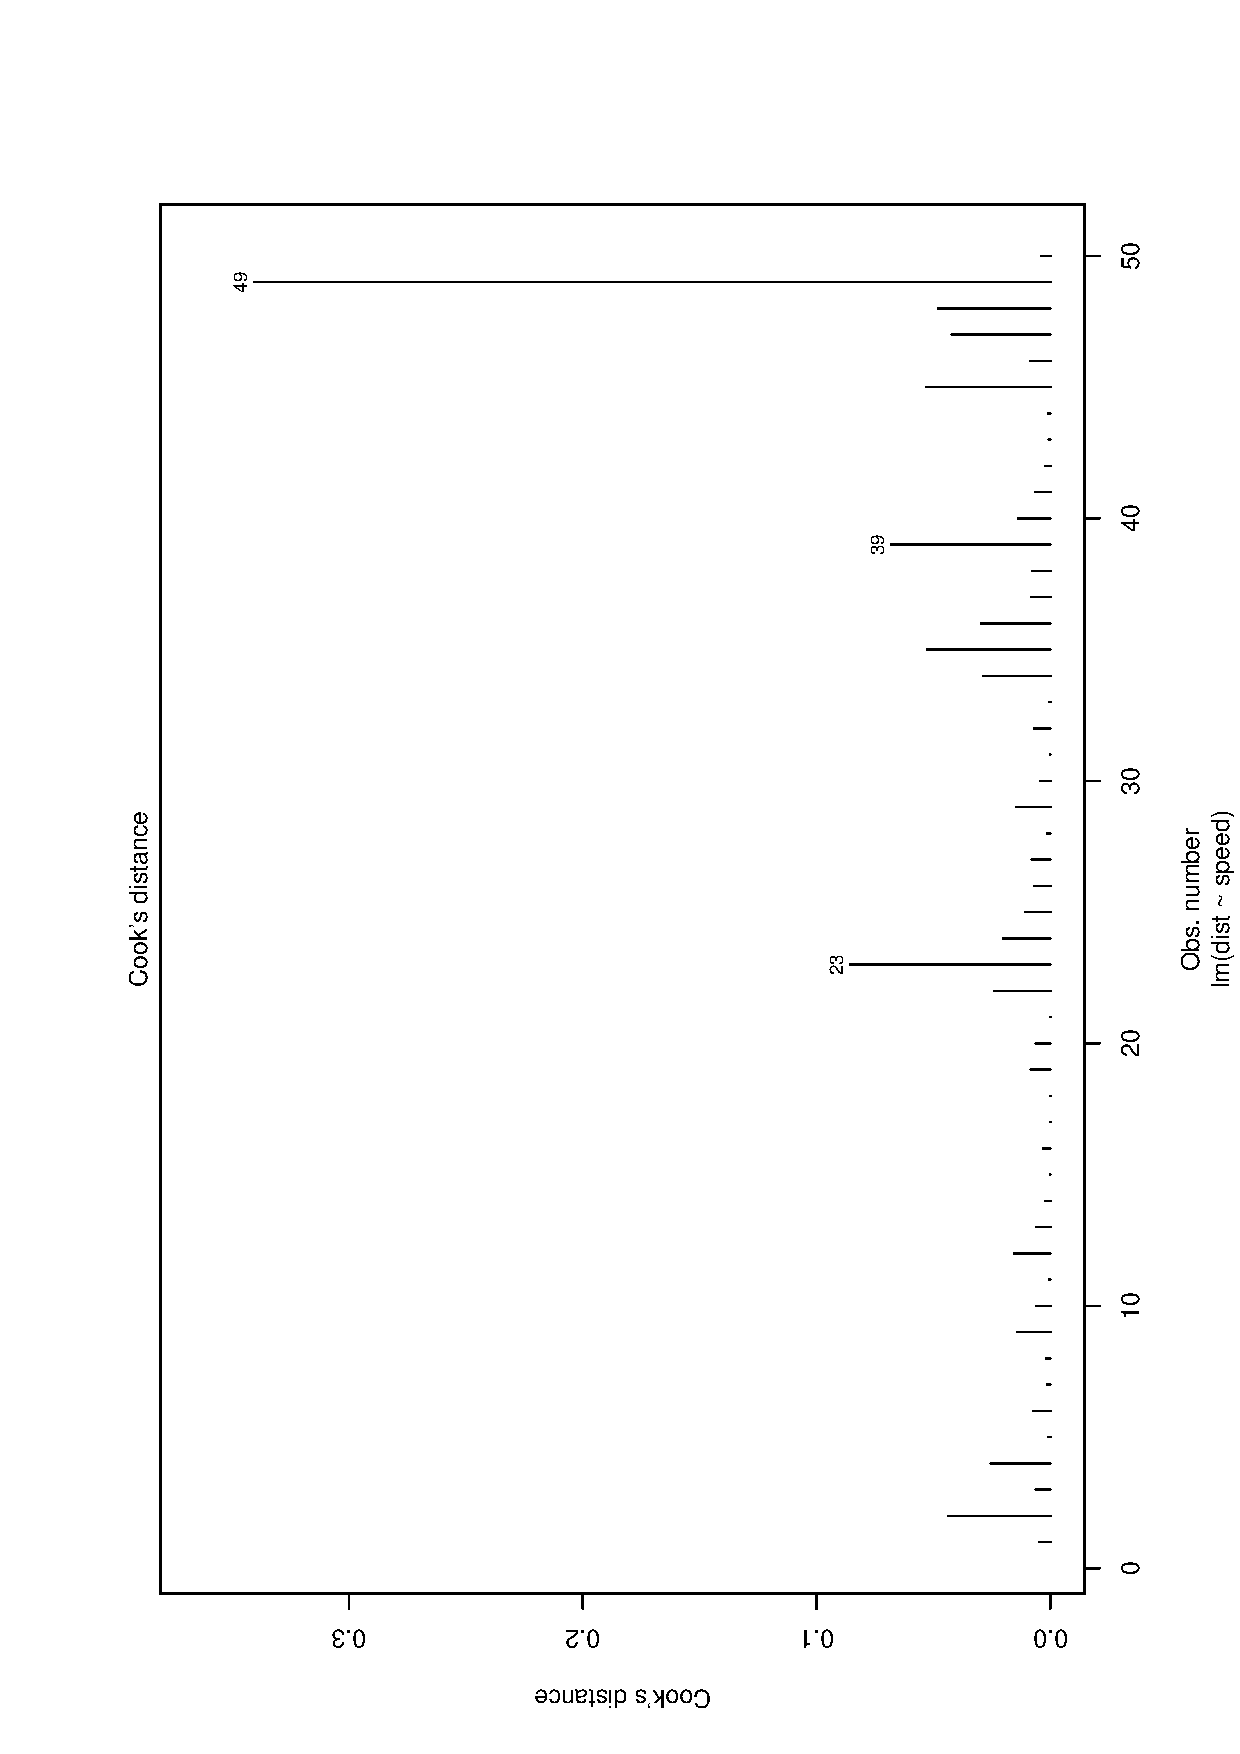
\includegraphics[width=5in, height=4in]{img/Cooks-distance-cars.pdf}
  \caption[Cook's distances for the \texttt{cars} data]{\small Used for checking for influential and/our outlying observations. Values with large Cook's distance merit further investigation.}
  \label{fig:Cooks-distance-cars}
\end{figure}


\begin{verbatim}
plot(cars.lm, which = 4)
\end{verbatim}

Observations with the largest Cook's D values are labeled, hence we see that observations 23, 39, and 49 are suspicious. However, we need to compare to the quantiles of an \( \mathsf{f}(\mathtt{df1} = 2, \, \mathtt{df2} = 48) \) distribution:


\begin{verbatim}
F0.50 <- qf(0.5, df1 = 2, df2 = 48)
any(cooksD > F0.50)
\end{verbatim}

\begin{verbatim}
 null device 
           1
 [1] FALSE
\end{verbatim}

We see that with this data set there are no observations with extreme Cook's distance, after all.
\subsection{All Influence Measures Simultaneously}
\label{sec-1-5-5}


We can display the result of diagnostic checking all at once in one table, with potentially influential points displayed. We do it with the command \texttt{influence.measures(cars.lm)}:


\begin{verbatim}
influence.measures(cars.lm)
\end{verbatim}

The output is a huge matrix display, which we have omitted in the interest of brevity. A point is identified if it is classified to be influential with respect to any of the diagnostic measures. Here we see that observations 2, 11, 15, and 18 merit further investigation.  

We can also look at all diagnostic plots at once with the commands


\begin{verbatim}
par(mfrow = c(2,2))
plot(cars.lm)
par(mfrow = c(1,1))
\end{verbatim}

The \texttt{par} command is used so that \(2\times 2 = 4\) plots will be shown on the same display. The diagnostic plots for the \texttt{cars} data are shown in Figure \ref{fig:Diagnostic-plots-cars}:

\begin{figure}[ht!]
  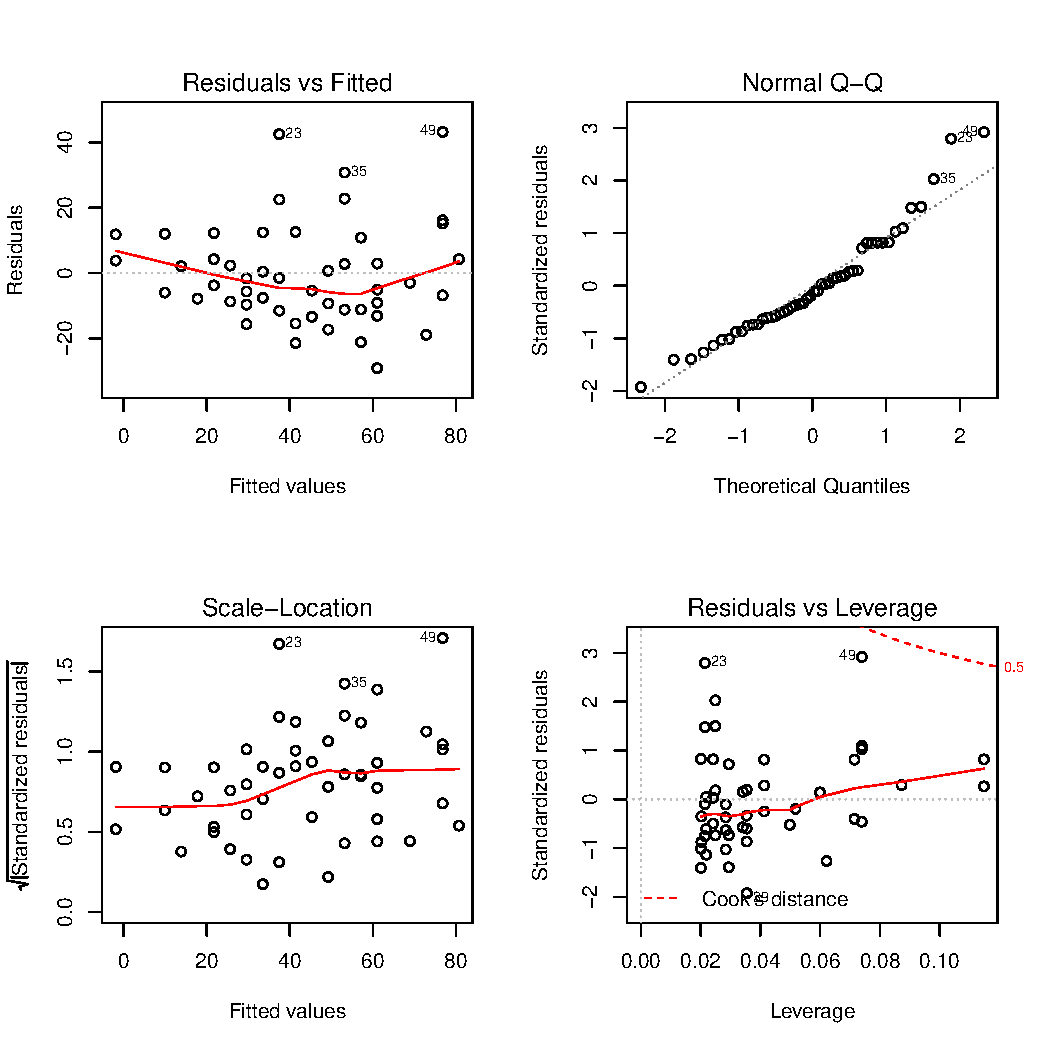
\includegraphics[width=5in, height=4in]{img/Diagnostic-plots-cars.pdf}
  \caption[Diagnostic plots for the \texttt{cars} data]{\small Diagnostic plots for the \texttt{cars} data.}
  \label{fig:Diagnostic-plots-cars}
\end{figure}



We have discussed all of the plots except the last, which is possibly the most interesting. It shows Residuals vs. Leverage, which will identify outlying \(y\) values versus outlying \(x\) values. Here we see that observation 23 has a high residual, but low leverage, and it turns out that observations 1 and 2 have relatively high leverage but low/moderate leverage (they are on the right side of the plot, just above the horizontal line). Observation 49 has a large residual with a comparatively large leverage. 

We can identify the observations with the \texttt{identify} command; it allows us to display the observation number of dots on the plot. First, we plot the graph, then we call \texttt{identify}:


\begin{verbatim}
plot(cars.lm, which = 5)   # std'd resids vs lev plot
identify(leverage, sres, n = 4)   # identify 4 points
\end{verbatim}

The graph with the identified points is omitted (but the plain plot is shown in the bottom right corner of Figure \ref{fig:Diagnostic-plots-cars}). Observations 1 and 2 fall on the far right side of the plot, near the horizontal axis.

\newpage{}
\section{Chapter Exercises}
\label{sec-1-6}


\addcontentsline{toc}{section}{Chapter Exercises}
\setcounter{thm}{0}

\begin{xca}
Prove the ANOVA equality, Equation \ref{eq:anovaeq}. \emph{Hint}:
show that
\[
\sum_{i=1}^{n}(Y_{i}-\hat{Y_{i}})(\hat{Y_{i}}-\overline{Y})=0.
\]
\end{xca}

\begin{xca}
\label{xca:find-mles-SLR}
Solve the following system of equations for \(\beta_{1}\) and \(\beta_{0}\) to find the MLEs for slope and intercept in the simple linear regression model.
\begin{eqnarray*}
n\beta_{0}+\beta_{1}\sum_{i=1}^{n}x_{i} & = & \sum_{i=1}^{n}y_{i}\\
\beta_{0}\sum_{i=1}^{n}x_{i}+\beta_{1}\sum_{i=1}^{n}x_{i}^{2} & = & \sum_{i=1}^{n}x_{i}y_{i}
\end{eqnarray*}
\end{xca}

\begin{xca}
\label{xca:show-alternate-slope-formula}
Show that the formula given in Equation \ref{eq:sample-correlation-formula} is equivalent to
\[
\hat{\beta}_{1} = \frac{\sum_{i=1}^{n}x_{i}y_{i}-\left.\left(\sum_{i=1}^{n}x_{i}\right)\left(\sum_{i=1}^{n}y_{i}\right)\right\slash n}{\sum_{i=1}^{n}x_{i}^{2}-\left.\left(\sum_{i=1}^{n}x_{i}\right)^{2}\right\slash n}.
\]
\end{xca}

\end{document}